\chapter{Photon Detection System}
\label{ch:dp-pds}

The \dword{pds} of the \dune \dual module uses large-area cryogenic \dwords{pmt} coated with \dword{tpb} to detect the \SI{127}{\nm} light produced by argon scintillation. The \dwords{pmt} are installed on the cryostat floor, underneath the \dshort{tpc} transparent cathode, and view the entire \lar volume of one \dword{fd} module. The design described in this chapter builds on experience from several \lartpc{}s, and particularly from the \dword{wa105} and from the \dword{pddp} detectors at \dshort{cern}. 

The chapter is organized as follows. Section~\ref{sec:dp-pds-requirements} introduces the physics requirements to be met by the \dword{pds}, and additional opportunities offered by the system. Section~\ref{sec:dp-pds-overview} gives gives an overview of the \dword{pds} baseline design, together with the detector specifications to be satisfied. Sections~\ref{sec:dp-pds-photosensors}--\ref{sec:dp-pds-calibration} describe in detail the \dword{pds} baseline design, and particularly the \dword{pds} photosensor system (Section~\ref{sec:dp-pds-photosensors}), the mechanical aspects (Section~\ref{sec:dp-pds-mechanics}),  the readout electronics (Section~\ref{sec:dp-pds-electronics}) and the calibration system (Section~\ref{sec:dp-pds-calibration}). Sections~\ref{sec:dp-pds-simulation}--\ref{sec:dp-pds-performance} demonstrate how the PDS baseline design has been validated using detailed simulations (Section~\ref{sec:dp-pds-simulation} and \ref{sec:dp-pds-performance}) and experience from prototypes (Section~\ref{sec:dp-pds-prototypes}). Sections~10-15 cover PDS project aspects, namely: quality control (Section~10), interfaces (Section~11), installation (Section~12), risks (Section~13), safety (Section~14), and high-level schedule and cost (Section~15). Finally, Section~16 discusses a limited number of alternatives to this baseline design.  

\section{Physics Requirements and Goals}
\label{sec:dp-pds-requirements}

The \dfirst{pds} of the \dshort{dune} \dword{fd} provides information on three key detection aspects of the experiment:

\begin{enumerate}
\item Event (and sub-event) time reconstruction.
\item Event triggering.
\item Event energy reconstruction.
\end{enumerate}

As discussed below, these detection aspects enabled by the \dshort{pds} affect the entire primary physics program of \dshort{dune}: long-baseline neutrino oscillations, nucleon decay, and supernova burst neutrinos. In the following, we list the scientific requirements to be met by the \dshort{pds} (Sec.~\ref{subsec:dp-pds-requirements_requirements}), as well as additional scientific opportunities offered by the \dshort{pds} (Sec.~\ref{subsec:dp-pds-requirements_opportunities}). Among requirements we only list the \dshort{pds} detection aspects that affect the \dshort{dune} primary physics program in a major way, namely: 
\begin{enumerate}
\item A capability or measurement uniquely provided by the \dshort{pds}.
\item A capability or measurement redundant with \dshort{tpc} information, but where redundancy is considered essential.
\item A capability or measurement competitive with \dshort{tpc} information.
\end{enumerate}

%%%%%%%%%%%%%%%%%%%%%%%%%%%%%%%%%%%%%%%%%%%%%%%%%%%%%%%%%%%%%%%%%%%%

\subsection{Scientific Requirements}
\label{subsec:dp-pds-requirements_requirements}

\subsubsection{Event fiducialization for non-beam events}

Absolute event time in the \dshort{dune} \dshort{tpc} is provided by the accelerator complex for beam events, but must be provided by the \dshort{pds} for non-beam events. Event time reconstruction is necessary to determine the drift distance within the \dshort{tpc}. This is essential for a number of reasons, and particularly for defining a fiducial volume along the \dshort{tpc} drift direction, which is the vertical one in the DP case. The cosmic ray (CR) activity in one FD module is of order \SI{0.05}{\Hz}, or about \SI{1e8}{\per(\Mtyr)}. Although smaller, the atmospheric neutrino event rate in one FD module is also significant, of order \SI{1e5}{\per(\Mtyr)}. These rates can be compared with the background levels aimed for nucleon decay (NDK) searches at \dshort{dune}. For the NDK channels where \dshort{dune} can provide the best sensitivities, the goal is to operate in nearly background-free conditions even after an exposure of several years, that is with background levels of order \SI{10}{\per(\Mtyr)} or less. Hence, the CR activity must be suppressed by at least seven orders of magnitude to enable optimal NDK searches. \dshort{pds} information is essential to reach the required levels of suppression of CR-induced (and atmospheric neutrino-induced) backgrounds. As most CR-activity will enter from the top of the detector, a NDK candidate must be required to be fully contained within the detector. For the most relevant direction, namely the vertical one, the fiducial requirement can only be imposed if \dshort{pds} information is available. As this capability is uniquely provided by the \dshort{pds} and since it critically affects the NDK program, {\bf we consider event fiducialization of nucleon decay candidates to be the most important requirement of the \dshort{pds}}. As high signal efficiency is critical in rare event searches such as NDK, {\bf we require a $\boldsymbol{>90\%}$ efficient event time determination via the \dshort{pds} throughout the \dshort{tpc} active volume for NDK signal events}. NDK event fiducialization may be prevented not only if NDK flashes are undetected, but also if the \dshort{pds} detects spurious flashes within the same event window, uncorrelated with the NDK activity. Additional flashes are produced, typically, by radiologically-induced detector activity. In this case, an ambiguity in the drift time determination of the nucleon decay may arise, and the correct (NDK-induced) flash must be associated to the event. Hence, {\bf we also require a $\boldsymbol{>90\%}$ NDK flash purity among all reconstructed NDK-like flashes within the same NDK event readout window}. Similarly, the \dshort{pds} is also needed to determine the full containment of atmospheric neutrino interactions in \dshort{dune}.
 
\subsubsection{Supernova burst triggering}

A burst of several hundred neutrino interactions per \dshort{dune} FD module is expected over a timescale of about \SI{10}{\s} from a core-collapse supernova at a \SI{10}{\kilo\parsec} distance from Earth, near the center of our galaxy. As the \dword{snb} interaction rate scales as $1/r^2$, where $r$ is the supernova distance from us, \dshort{snb} detection at \dshort{dune} is in principle possible up to distances of order \SI{50}{\kilo\parsec}. This would be the case for an \dshort{snb} occurring in the Large Magellanic Cloud, for example. The dominant neutrino interaction channel in \dshort{dune} is the \dword{cc} electron neutrino interaction on an argon nucleus, with typical deposited energies from electrons and nuclear de-excitation gammas of order 20~MeV, producing short tracks throughout the \dshort{tpc} active volume.

In \dshort{dune}, one can in principle trigger on \dshort{snb}s using either \dshort{tpc} or \dshort{pds} information. In both cases, the trigger scheme exploits the time coincidence of multiple signals (\dshort{tpc} stubs or \dshort{pds} flashes) over a timescale matching the SN luminosity time evolution. In the case of an \dshort{snb} trigger being generated, the data acquisition system would write to disk the full (non-zero-suppressed) detector information for a time range spanning several tens of seconds surrounding the trigger timestamp. Considering the rare nature of \dshort{snb}s in our galactic neighbourhood, and given the importance of \dshort{snb} detection, we consider essential to develop both a redundant and a highly efficient \dshort{snb} triggering scheme in \dshort{dune}. Concerning redundancy, {\bf we require that the \dshort{dune} FD may trigger on an \dshort{snb} independently using \dshort{tpc} or \dshort{pds} information}, hence minimising \dshort{snb} inefficiencies stemming from downtime or malfunctioning of the \dshort{tpc}, the \dshort{pds} or their associated trigger schemes. As for trigger efficiency, {\bf we require the \dshort{pds} alone to be able to trigger with $\boldsymbol{>90\%}$ efficiency on a \dshort{snb} at a \SI{20}{\kilo\parsec} distance from Earth}, hence up to distances covering the entire Milky Way. Considering the very large amount of detector information being generated by a \dshort{snb} trigger, we also require that such \dshort{snb} trigger efficiency can reached for a {\bf fake trigger rate not exceeding \SI{1}{\per month}}.

\subsubsection{Scintillation-based calorimetry}

The most important physics goal of the \dshort{dune} FD is to carry out a comprehensive program of neutrino oscillation measurements using \numu and \anumu beams from Fermilab. Because of this, the \dshort{dune} FD performance in terms of neutrino energy reconstruction and neutrino flavour classification is of paramount importance. As detailed in this volume, the \dshort{tpc} is expected to provide a 10--15\% neutrino energy resolution for \nue \dshort{cc} interactions in the few-GeV energy range, using charge information alone. At these energies, however, thousands of PEs are also going to be detected by the \dshort{pds}. Thus, a competitive calorimetric measurement of the event energy can in principle be obtained also using the light intensity detected by the \dshort{pds}, provided that spatial non-uniformities in \dshort{pds} response can largely be corrected for. {\bf We require the \dshort{pds} alone to be able to reconstruct the neutrino energy of a few-GeV electron neutrino \dshort{cc} interaction with 20\% RMS resolution or better}, hence providing a competitive measurement with respect to the \dshort{tpc}-based one. Such an independent and competitive energy measurement would also be useful as a risk mitigation measure for degraded \dshort{tpc} performance. The \dshort{tpc}- and \dshort{pds}-based energy measurements may be combined together, possibly providing better energy resolution with respect to the \dshort{tpc} alone. We give two arguments supporting this possibility. On the one hand, the charge and light signals may be combined to reduce electron-ion recombination fluctuations, ensuring a more compensating \dshort{lar} calorimeter response. On the other hand, charge and light readout planes are located at opposite detector ends in the DP design, providing maximal complementarity between the two. Neutrino interactions occurring near the light readout at the bottom of the cryostat will be maximally affected by electron attachment of the charge signal, while they will have the highest light detection probabilities possible. The situation is reversed for neutrino interactions near the charge readout plane. The \dshort{pds} may provide a competitive energy measurement not only for beam neutrinos, but also at lower energies, particularly for \dshort{snb} neutrinos. For a discussion of why an accurate energy measurement is beneficial also for \dshort{snb} events, see Sec.~\ref{subsubsec:dp-pds-requirements_attachment}.

%%%%%%%%%%%%%%%%%%%%%%%%%%%%%%%%%%%%%%%%%%%%%%%%%%%%%%%%%%%%%%%%%%%%

\subsection{Additional Scientific Opportunities}
\label{subsec:dp-pds-requirements_opportunities}

\subsubsection{Electron attachment correction for the charge-based energy measurement in non-beam events}
\label{subsubsec:dp-pds-requirements_attachment}

Given the maximum drift distance of \dpmaxdrift in the DP \dshort{tpc} and assuming a (minimally-required) \SI{3}{\ms} electron lifetime, the charge could be attenuated by more the one order of magnitude along drift due to electron attachment on electro-negative impurities. If left uncorrected, electron attachment would therefore greatly deteriorate the charge-based energy measurement in the case of such relatively short electron lifetimes. Because of the longer drift distance, this effect is much more dramatic in the DP compared to the SP case. For non-beam events, the only possible way of correcting for the electron attachment is via \dshort{pds}-based event timing\footnote{This is true for a single physics event (\emph{e.g.}, a neutrino interaction) per \dshort{tpc} event. Neglecting background flashes, there are no ambiguities in the association between \dshort{tpc} tracks and \dshort{pds} flashes in this case.}. This will be exploited in \dshort{dune} to better discern, for example, the spectral features in the energy spectrum of the \dshort{snb} flux. An improved charge-based energy measurement would improve both the determination of the pinched-thermal spectral parameters of the progenitor, as well as the detection of the sharp, time-dependent spectral features from collective neutrino oscillations. A similar argument applies to the charge-based energy measurement in the study of atmospheric neutrino oscillations, where good neutrino energy reconstruction is also very important.

\subsubsection{Event timing in high multiplicity supernova burst events}

The early time distribution carries important information for core-collapse stellar models, one that has not been observed thus far. The first neutrino release after core bounce is the \nue-rich neutronization burst, lasting about \SI{10}{\ms}. For a supernova at a \SI{10}{\kilo\parsec} distance, several tens of interactions induced by the neutronization flux should be detected in one FD module. In other words, the mean interval between successive neutrino interactions is expected to be less than \SI{1}{\ms} in this case. For closer supernovae, information at even earlier (pre-bounce) times may be studied, during the core infall phase. A \SI{1}{\ms} wide notch in the luminosity curve may be visible, corresponding to neutrino trapping in the ultra-dense matter. Such timescales can be compared with the typical time resolutions that can be obtained with \dshort{tpc} and \dshort{pds} information. In the DP \dshort{tpc} case, the drift time can be as large as \SI{7.5}{\ms}, with foreseen readout windows of \dpreadout. Considering the uniform spatial distribution of neutrino interactions in the \dshort{tpc}, the intrinsic absolute time resolution expected in this case is therefore of order $\dpreadout/\sqrt{12}\simeq \SI{5}{\ms}$. The \dshort{tpc}-based time resolution is therefore not sufficient to resolve these early time features, even in the case of sufficient neutrino statistics. On the other hand, the \dshort{pds} may reconstruct one flash per \dshort{snb} neutrino interaction with \SI{1}{\micro\s}-scale time resolution. Hence, \dshort{pds}-based timing is a definite added value in the occurrence of a nearby supernova.

\subsubsection{Improved event identification via scintillation-based Michel electron tagging}

There is another physics case where the \dshort{pds} may detect more than one physics-induced flash per \dshort{tpc} event\footnote{We use the qualifier 'physics-induced' to distinguish those light flashes from the ones induced by radiological or cosmogenic activity in the detector, or by electronics noise.}. This can happen in the presence of particle decays in the final state of an event of interest, such as a neutrino interaction or a nucleon decay. In this case, multiple, correlated sub-events may be separated in time. Michel electron tagging from muon decay at rest represents the most obvious opportunity for sub-event identification via \dshort{pds} timing. Approximately one million scintillation photons are produced in the liquid argon per Michel electron. In addition, the timescale of muon decay is long, comparable to the timescale of the slow component of argon scintillation light. While Michel electrons can be identified also through \dshort{tpc} track imaging, there are event topologies where \dshort{pds} may outperform the \dshort{tpc}, for example in the case where the muon and electron tracks are nearly parallel. In summary, the \dshort{pds} may provide a better identification of the event final state, compared to \dshort{tpc}-only information. Considering the large fraction of $\mu^-$ capture on argon (about 75\%), Michel electron tagging also provides valuable $\mu^-/\mu^+$ separation. The latter can, in turn, provide separation between muon neutrinos and antineutrinos. 

\section{Design Overview}
\label{sec:dp-pds-overview}

The \dual \dword{pds} is optimized for the physics program of the full-size \dune \dual detector. Phenomena leading to interactions in the \dword{dune} detectors and to be studied span several orders of magnitude of energy scale, from a few \si{MeV} to several \si{GeV}, with commensurate range in light yield. In particular, low-energy signals like \dword{snb} neutrinos and proton decay, impose more stringent requirements on \dword{pds} performance than the primarily higher energy, beam-synchronous, neutrino oscillations physics.

%A number of scientific and technical choices and issues impact the \dual \dword{pds}  and \single \dword{pds}  in a similar way, so the consortia for these two systems cooperate closely.  %See \voltitlespfd{}, Chapter 5 for details on the \single \dword{pds}.

%%%%%%%%%%%%%%%%%%%%%%%%%%%%%%%%%

\subsection{Scintillation Light Production in the \dual Detector Module}
\label{sec:dp-pds-overview_scintillation}

\dual \dword{pds} detects light produced from two sources: the scintillation process originated by ionizing particles propagating in the liquid argon (usually referred to as the S1 signal) and by the electroluminescence process due to drift electrons extracted from the liquid phase and accelerated in the argon vapor at the top of the cryostat (usually referred to as the S2 signal). Charge readout anode planes instrument the top while photodetectors are at the bottom of the cryostat. The interplay between the charge and light from an event enables pattern recognition and measuring the energy of interactions.

Ionizing radiation in liquid noble gases leads to the formation of excimers in either singlet or triplet states, which decay radiatively to the dissociative ground state with characteristic S1 fast and slow lifetimes (fast is approximately \SI{6}{ns} and slow approximately \SI{1.3}{$\mu$s} in \lar with the so-called second continuum emission spectrum peaked at the wavelength of approximately \SI{127}{nm}, \SI{126.8}{nm} with a full width at half maximum of \SI{7.8}{nm} \cite{Heindl}). This prompt and relatively high-yield (about \num{40000} photons per \si{MeV} at zero \efield) of \SI{127}{nm} scintillation light is exploited in an \lartpc (both \dshort{dp} and \dshort{sp}) to provide the absolute time ($t_0$) of the ionization signal collected at the anode, thereby providing the absolute value of the drift coordinate of fully contained events and a prompt signal used for triggering. Figure~\ref{fig:dppd_6_0} shows the light production mechanism in \lar.

\begin{dunefigure}[A sketch depicting the mechanism of light production in argon.]{fig:dppd_6_0}
{A sketch depicting the mechanism of light production in argon.}
\includegraphics[width=0.95\textwidth]{dppd_6_0}
\end{dunefigure}

The secondary scintillation in the argon gas (i.e., the vapor phase) is unique to the \dpmod technology. It is the luminescence in gas caused by accelerated electrons in the \efield and in the \dword{lem} anode through Townsend amplification. The S2 signal provides information on the drift time and amount of ionization charge, thus supplementing information from the charge readout on the anode plane. For a given argon gas density, the number of S2 photons is proportional to the number of electrons, the \efield, and the length of the drift path in gas covered by the electrons. In an extraction field of \SI{3.0}{kV/cm} in gas, one electron generates about \num{100} downward-moving photons that cross the liquid argon surface \cite{Lux:2018zwd}. The time scale of S2 reflects the extraction time of original ionization from the liquid phase into the gas phase. Therefore, for about \SI{0.5}{kV/cm} drift \efield, this time scale is of the order of hundreds of microseconds. The time between the occurrence of the primary scintillation light and the secondary scintillation light is equivalent to the drift time of the electrons from the ionization coordinate to the \lar surface. This provides an accurate determination of the drift time in the active volume and, hence, a correction tool for the electron attachment (and the associated energy measurement).  


%The chapter begins with an overview of the system in Section~\ref{sec:fddp-pd-1}. Section~\ref{sec:fddp-pd-2} describes the photosensors, namely \dwords{pmt} %tubes  
%and the related \dword{hv} system, wavelength shifters and light collectors. The mechanics associated with the \dwords{pmt} is described in Section~\ref{sec:fddp-pd-3}, and the readout electronics in~\ref{sec:fddp-pd-4}. Section~\ref{sec:fddp-pd-5} details the photon calibration system to monitor the \dword{pmt} gain and stability. Then, the \dword{pd} performance is described in Section~\ref{sec:fddp-pd-6}, and the operations in Section~\ref{sec:fddp-pd-7}. Interfaces with other subsystems are described in Section~\ref{sec:fddp-pd-8}. Section~\ref{sec:fddp-pd-9} includes the installation, integration and commissioning plans. The \dword{qc} procedures are outlined in Section~\ref{sec:fddp-pd-10}. The main safety issues to consider are specified in Section~\ref{sec:fddp-pd-11}. To finish, the management and organization is described in Section~\ref{sec:fddp-pd-12}.

%%%%%%%%%%%%%%%%%%%%%%%%%%%%%%%%%
\subsection{Detector Sub-systems and Layout}
\label{sec:dp-pds-overview_layout}

The baseline design of the light collection system calls for \SI{20.3}{cm} (\SI{8}{in}) diameter cryogenic \dwords{pmt} from Hamamatsu Photonics\footnote{Hamamatsu Photonics\texttrademark{}, \url{http://www.hamamatsu.com/resources/pdf/etd/LARGE_AREA_PMT_TPMH1286E.pdf}} (model R5912-MOD20) distributed uniformly on the floor (bottom) of the cryostat and electrically shielded from the bottom cathode plane. Other \dword{pmt} manufacturers being considered include Electron Tubes Limited~\footnote{Electron Tubes Ltd\texttrademark{}, \url{http://www.electron-tubes.co.uk//}} and HZC~\footnote{HZC Photonics\texttrademark{}, \url{http://hzcphotonics.com/en_index.html}.}. According to the baseline design, \dpnumpmtch \dwords{pmt}, approximately \num{1} per \si{m$^2$}, will be installed. The outline of the \dword{dpmod} is shown in Figure~\ref{fig:dppd_3_1}.

\begin{dunefigure}[The \dword{dpmod} (partly open)]{fig:dppd_3_1}
{The \dword{dpmod} (partly open) with cathode, \dwords{pmt}, \dword{fc}, and anode plane with chimneys.}
%\includegraphics[width=0.95\textwidth]{dppd_3_1}
%\includegraphics[width=0.95\textwidth]{dppd_1_1_v2}
\includegraphics[width=0.95\textwidth]{dppd_1_1_v3}
\end{dunefigure}

The \dwords{pmt} are individually powered to values between \num{1.5} to \num{2.0} \si{\kV} to separately adjust the \dword{pmt} gains. The Hamamatsu R5912 \dwords{pmt} are not sensitive to the \SI{127}{nm} scintillation light, so a wavelength shifter is required. A thin layer of \dword{tpb}~\cite{tpb} coating is applied directly on the \dword{pmt} window by evaporation. Section~\ref{sec:dp-pds-photosensors} describes the photosensor system.

The \dpnumpmtch \dwords{pmt} are individually attached to the cryostat floor \SI{1.02}{m} apart in both directions, via a \dword{pmt} support structure that counteracts the \dword{pmt} buoyancy. In order to enhance the light collection and to improve the photon detector response uniformity throughout the entire \dword{tpc} active volume, \dword{tpb} coated reflector/\dword{wls} panels will be installed on the top half of the \dword{fc} inner surfaces. Considering the linear relationship between the number of \dwords{pmt} and the detected light yield, and the mild dependence of the \dword{pds} physics performance on light yield and channel granularity, the optimization process that resulted in this baseline design can be considered very robust. The mechanical aspects of the \dword{pmt} support structures and the reflector/\dword{wls} assemblies are described in Section~\ref{sec:dp-pds-mechanics}.

The front-end \dword{pmt} base circuit for reading the photo-electron signals relies on a positive \dword{hv} supplied to the \dword{pmt} anode and on a grounded photo-cathode. A single cable for each \dword{pmt} carries both power and signal. \dword{hv} and signal splitters located outside the cryostat separate the fast \dword{pmt} response signal from the positive \dword{hv} with capacitive decoupling. The \dword{pds} readout electronics is described in Section~\ref{sec:dp-pds-electronics}.

A photon calibration system is required to determine the \dword{pmt} gain and to monitor the stability of the \dword{pmt} response. The LED-driven fiber calibration system of the \dword{pds} is described in Section~\ref{sec:dp-pds-calibration}. 

The basic unit of installation/operation is called a sector. The sectors are indicated as transparent red and yellow panels in Figure~\ref{fig:dppd_3_1}. One \dual \dword{pds} sector is \SI{6}{\m} $\times$ \SI{6}{\m} and houses \num{36} \dwords{pmt}. A total of \num{20} sectors will be installed in the detector. A single \dword{hv} cable per \dword{pmt} will be installed in the cryostat.
%The cables from the \dword{pmt} locations (RG303/U) will run in bundles at the cryostat floor to either side. The short cables attached to the \dword{pmt} bases will be connected to these long cables during the \dword{pmt} installation at the cryostat floor. The long cables from each sector will be bundled and will run through a cable tray along the \SI{12}{\m} side wall to the top of the cryostat. 
The cable trays for the two sectors in Figure~\ref{fig:dppd_3_1} are indicated as black vertical lines.
%The single cable density is approximately \SI{50}{\g/\m}. The cable length at the cryostat floor will be \SI{9}{\m} (determined by the farthest \dwords{pmt}), the side wall length is \SI{12}{\m}, and the additional average cable length per \dword{pmt} is estimated to be \SI{4}{\m}. Therefore, the overall cable length per \dword{pmt} is \SI{25}{\m}. This corresponds to approximately \SI{2}{\kg/\m} load on the cable trays on the side walls (a total of \SI{24}{\kg} assuming a cable density of \SI{50}{\g/\m}) per sector, also including the \num{6} calibration fibers. 

The high voltage cables will penetrate a feedthrough flange and end with SHV connectors, with the calibration fibers also penetrating a feedthrough flange and end with SMA connectors. One DN250 flange is used per sector of \dual \dword{pds}. One flange will house \num{36} SHV and \num{6} SMA connections. The \dual \dword{pds} design will have \num{20} penetrations on the cryostat roof, one per sector. 

The high voltage and signal crates will be at a density of one per sector for a total of \num{20} \dword{hv}/signal racks on the cryostat roof. Figure~\ref{fig:dppd_1_2} illustrates the layout of the feedthroughs and the \dword{hv}/signal/calibration racks for four sectors. The racks will contain the \dword{hv} crates, \dword{hv}/signal splitters, the \dword{utca} crates for the front-end electronics, and the calibration LED driver and the associated electronics for \num{36} \dwords{pmt}.

\begin{dunefigure}[The sketch of the cryostat roof layout for \dual \dword{pds} penetrations.]{fig:dppd_1_2}
{The sketch of the cryostat roof layout for \dual \dword{pds} penetrations.}
%\includegraphics[width=0.95\textwidth]{dppd_3_1}
\includegraphics[width=0.55\textwidth]{dppd_1_2}
\end{dunefigure}

The cathode plane, described in Chapter~\ref{ch:dp-hv}, is placed approximately \SI{2}{m} above the bottom of the cryostat. Given the high dielectric constant of the \lar phase, the \dword{pmt} plane is a safe distance from the cathode plane. To protect the \dwords{pmt}, the ground grid is installed and placed at an identical potential as the \dword{pmt} photocathode (\SI{0}{V}).

%%%%%%%%%%%%%%%%%%%%%%%%%%%%%%%%%
\subsection{Operational Modes} %Principles}
\label{sec:dp-pds-oveerview_operation}

The physics program defines the operational modes of the \dual \dword{pds}. Measuring the neutrino oscillation parameters requires recording events upon receiving an external trigger from the beam, while non-beam physics such as \dwords{snb}, proton decay, or other rare events require special trigger conditions that include the \dword{pds}. Another operation mode is the \Dword{pmt} calibration run, which is initiated by the light calibration system with its dedicated hardware trigger.
%
Thus, the operation modes are
\begin{itemize}
\item External trigger: %this is mainly the case of 
A typical case is when the beam generates a hardware trigger (a beam gate);  it also includes software-generated triggers for test data.
\item Non-beam physics trigger: The electronics based on the \dword{pds} signals provides the trigger for, among other events, \dword{snb} and proton decay events;
\item Calibration trigger: The trigger is provided by the light calibration system during \dword{pds} calibrations.
\end{itemize}

The external and non-beam physics triggers run in parallel to ensure that rare events like \dwords{snb} are recorded efficiently. 

%%%%%%%%%%%%%%%%%%%%%%%%%%%%%%%%%
\subsection{Detector Design Specifications}
\label{sec:dp-pds-overview_specs}

The \dual \dword{pds} detector specifications are given in Table~\ref{tab:specs:just:DP-PDS}. The physics-driven rationale for each detector specification, and the means to validate them, are also summarized in the table. Validation of the detector specifications uses data from \dword{pds} prototypes (Section~\ref{sec:dp-pds-prototypes}) and from a full simulation/reconstruction of signal and background optical flashes in the \dpmod (Section~\ref{sec:dp-pds-performance}). 

%\fixme{(from Anne) Here is your requirements table. For SP, we've asked each chapter to include the "top 5" of the FD specs. That may not be appropriate for DP, since those top-level specs (approved by EB) may not exist yet.}

%% This file is generated, any edits may be lost.
\begin{footnotesize}
%\begin{longtable}{p{0.14\textwidth}p{0.13\textwidth}p{0.18\textwidth}p{0.22\textwidth}p{0.20\textwidth}}
\begin{longtable}{p{0.12\textwidth}p{0.18\textwidth}p{0.17\textwidth}p{0.25\textwidth}p{0.16\textwidth}}
\caption{DP PDS specifications \fixmehl{ref \texttt{tab:spec:DP-PDS}}} \\
  \rowcolor{dunesky}
       Label & Description  & Specification \newline (Goal) & Rationale & Validation \\  \colhline

   \newtag{DP-FD-3}{ spec:dp-light-yield }  & Light yield  &  $>\,\SI{1}{PE/MeV}$ (min), $>\,\SI{3}{PE/MeV}$ (avg) \newline ($>\,\SI{5}{PE/MeV}) &  Enable  fiducialization of NDK candidates anywhere in active volume with $>90\%$ flash reconstruction efficiency and $>90\%$ purity. Enable SNB triggering efficiency of $>90\%$ in galaxy with a fake trigger rate $<$1/month. &  Supernova and nucleon decay events in the FD with full simulation and reconstruction. \\ \colhline
    
   \newtag{DP-FD-4}{ spec:dp-time-resolution-pds }  & Time resolution  &  $<\,\SI{1}{\micro\second}$ \newline ($<\,\SI{100}{\nano\second}$) &  Enables \SI{1}{mm} position resolution for \SI{10}{MeV} SNB candidate events for instantaneous rate $<\,\SI{1}{m^{-3}ms^{-1}}$. &   \\ \colhline
    
   
  \newtag{DP-FD-15}{ spec:dp-lar-n-contamination }  & LAr nitrogen contamination  &  $<\,\SI{25}{ppm}$ &  Maintain \SI{0.5}{PE/MeV} PDS sensitivity required for triggering proton decay near cathode. &   \\ \colhline
    

   
  \newtag{DP-PDS-1}{ spec:dp-light-yield }  & Light yield  &  $>\,\SI{1}{PE/MeV}$ at anode, $>\,\SI{5}{PE/MeV}$ avg over  active vol &  Enable drift position determination of \dword{ndk} candidates. Enable \dword{pds}-based triggering on galactic \dwords{snb}. &  Full sim/reco of \dword{ndk}, \dword{snb} $\nu$ and radiological events. \\ \colhline
    
   \newtag{DP-PDS-2}{ spec:dp-time-resolution }  & Time resolution  &  $<\,\SI{1}{\micro\second}$ \newline ( $<\,\SI{100}{\nano\second}$ ) &  Enables \SI{1}{mm} pos resolution for \SI{10}{MeV} \dwords{snb} candidate events for instantaneous rate $<\,\SI{1}{m^{-3}ms^{-1}}$. &   \\ \colhline
    
   
  \newtag{DP-PDS-3}{ spec:dp-lar-nitrogen-contamination }  & LAr nitrogen contamination  &  $<\,\SI{3}{ppm}$ &  Higher contaminations signifcantly affect the no. of photons that reach the \dword{pmt}. &   \\ \colhline
    
   
  \newtag{DP-PDS-4}{ spec:hit-relative-timing }  & Relative timing accuracy among hits  &  $<\,\SI{100}{ns RMS}$ &  Enable effective clustering of \dword{pmt} signals based on relative hit timing information. &  Full sim/reco of \dword{ndk}, \dword{snb} $\nu$ and radiological events. \\ \colhline
    


\label{tab:specs:DP-PDS}
\end{longtable}
\end{footnotesize}

%\fixme{The next table is just the DP PDS. It doesn't include the two SP FD requirements you selected (3 and 15 I think).}
% This file is generated, any edits may be lost.

\begin{longtable}{p{0.14\textwidth}p{0.13\textwidth}p{0.18\textwidth}p{0.22\textwidth}p{0.20\textwidth}}
\caption{Specifications for DP-PDS \fixmehl{ref \texttt{tab:spec:DP-PDS}}} \\
  \rowcolor{dunesky}
       Label & Description  & Specification \newline (Goal) & Rationale & Validation \\  \colhline

   
  \newtag{DP-PDS-1}{ spec:dp-light-yield }  & Light yield  &  $>\,\SI{1}{PE/MeV}$ at anode, $>\,\SI{5}{PE/MeV}$ avg over  active vol &  Enable drift position determination of \dword{ndk} candidates. Enable \dword{pds}-based triggering on galactic \dwords{snb}. &  Full sim/reco of \dword{ndk}, \dword{snb} $\nu$ and radiological events. \\ \colhline
     % 1
   \newtag{DP-PDS-2}{ spec:dp-time-resolution }  & Time resolution  &  $<\,\SI{1}{\micro\second}$ \newline ( $<\,\SI{100}{\nano\second}$ ) &  Enables \SI{1}{mm} pos resolution for \SI{10}{MeV} \dwords{snb} candidate events for instantaneous rate $<\,\SI{1}{m^{-3}ms^{-1}}$. &   \\ \colhline
     % 2
   
  \newtag{DP-PDS-3}{ spec:dp-lar-nitrogen-contamination }  & LAr nitrogen contamination  &  $<\,\SI{3}{ppm}$ &  Higher contaminations signifcantly affect the no. of photons that reach the \dword{pmt}. &   \\ \colhline
     % 3
   
  \newtag{DP-PDS-4}{ spec:hit-relative-timing }  & Relative timing accuracy among hits  &  $<\,\SI{100}{ns RMS}$ &  Enable effective clustering of \dword{pmt} signals based on relative hit timing information. &  Full sim/reco of \dword{ndk}, \dword{snb} $\nu$ and radiological events. \\ \colhline
     % 4
   
  \newtag{DP-PDS-5}{ spec:pmt-dark-rate }  & PMT dark count rate  &  $<\,\SI{100}{kHz}$ &  Dark counts should have negligible effect on clustering algorithm and PDS-based calorimetry. &  Characterization of PMTs at cryogenic temperatures prior to installation. \\ \colhline
     % 5
   
  \newtag{DP-PDS-6}{ spec:pds-analog-range }  & Analog range per channel  &  $>\,\SI{100}{PE/(channel\times 6\nano\second)}$ &  Minimize hit saturation for scintillation-based calorimetry in beam neutrino interactions over characteristic 6 ns time of prompt scintillation light production. &  Full simulation/reconstruction of beam $\nu$ interactions.  \\ \colhline
     % 6
   
  \newtag{DP-PDS-7}{ spec:pds-analog-range }  & Analog range per channel  &  $>\,\SI{100}{PE/(channel\times 6\nano\second)}$ &  Minimize hit saturation for scintillation-based calorimetry over \SI{6}{ns} prompt light period, esp. for beam events. &  Full sim/reco of beam $\nu$ interactions.  \\ \colhline
     % 7


\label{tab:specs:just:DP-PDS}
\end{longtable}

\section{Photosensor System}
\label{sec:dp-pds-photosensors}

The baseline photodetector for the light readout is the Hamamatsu R5912-MOD20 \dword{pmt}. This is the same model used in \dword{pddp}. The Hamamatsu R5912-MOD20, depicted in  Figure~\ref{fig:dppd_2_1}, is an 8-inch diameter, 14-stage, high gain \dword{pmt} (nominal gain of \num{e9}). The maximum quantum efficiency of the R5912-MOD20 \dword{pmt} is approximately \SI{20}{\%} at \SI{400}{\nano\m}. In addition, this \dword{pmt} was designed to work at cryogenic temperatures by adding a thin platinum layer between the photocathode and the borosilicate glass envelope to preserve the conductance of the photocathode at low temperatures. This particular \dword{pmt} has proved reliable in other cryogenic detectors. The same or similar \dwords{pmt} have successfully operated in other \lar experiments like MicroBooNE~\cite{microboone}, MiniCLEAN \cite{miniclean}, ArDM, ICARUS T600 \cite{icarus}, and \dword{pddp}~\cite{protoDUNDP-tdr}. Discussions with other manufacturers like Electron Tubes Limited (UK) \cite{electrontubeslim} and HZC (China) \cite{hzc} are on-going to include them in the program.

\begin{dunefigure}[Picture of the Hamamatsu R5912-MOD20 \dword{pmt}.]{fig:dppd_2_1}
{Picture of the Hamamatsu R5912-MOD20 \dword{pmt} \cite{hamamatsu-5912}.}
\includegraphics[width=0.3\textwidth]{dppd_2_1}
\end{dunefigure}

The baseline number of \dwords{pmt} is \dpnumpmtch with \num{80} spares.  Several operations and tests must be performed with the \dwords{pmt} before they are installed. The \dwords{pmt} must be ordered with sufficient lead time to complete the following planned operations: assembling the voltage divider circuit, mounting on the support structure, testing at room and cryogenic temperatures, packing and shipping to the \dword{ctsf}. The \dword{tpb} coating of the \dword{pmt} windows will be done at the \dword{ctsf}. The \dwords{pmt} will be re-tested for validation of basic functionality at the \dword{ctsf} and at \surf before installation (see Section~\ref{sec:dp-pds-installation}). Considering the large number of \dwords{pmt} required by \dual \dword{pds}, the purchase order must be completed at least two years before installation. A staged or staggered order with a steady supply of \dwords{pmt} would be most convenient and will be negotiated with the manufacturer.

%%%%%%%%%%%%%%%%%%%%%%%%%%%%%%%%%
\subsection{Photodetector Characterization}
\label{sec:dp-pds-selection-characterization}

Before installation, the most important characteristics of the \dword{pmt} response must be determined with two goals: to possibly reject under-performing \dwords{pmt} and to store the characterization information in a database for later use during the \dword{dpmod} commissioning and operation.

The basic and most important parameters to characterize are the dark count rate versus high voltage and the gain versus high voltage. Both parameters must be measured at room and cryogenic temperatures. As with the baseline \dword{pmt} model, the rates of pre-pulsing and after-pulsing should be negligible, but they will be measured as part of testing. 

From the mechanical point of view, the test set up requires a light-tight dark vessel filled with cryogenic liquid (argon or nitrogen) and an infrastructure for filling and operating the vessel with temperature and liquid-level controls. For \dword{pddp}, \num{10} \dwords{pmt} were tested at a time over a week because cryogenic tests of \dwords{pmt} require several days for \dword{pmt} thermalization \cite{Belver:2018erf}. Figure~\ref{fig:dppd_2_2a} shows the  \dword{pddp} \dwords{pmt} being installed in the testing vessel.
Increasing the capacity of the vessel, and thus the number of \dwords{pmt} that can be tested simultaneously,
could reduce the duration of the characterization test per \dword{pmt}.

\begin{dunefigure}[Picture of the \dwords{pmt} being installed in the testing vessel]{fig:dppd_2_2a}
{Picture of the \dwords{pmt} being installed in the testing vessel used for the \dword{pddp} \dwords{pmt}.}
\includegraphics[width=0.3\textwidth]{dppd_2_2a}
\end{dunefigure}

Figure~\ref{fig:dppd_2_2b} shows a sketch of the proposed set up for \dword{pmt} characterization tests. For the electronics, the test set up requires an \dword{hv} power supply, a discriminator, a counter for the dark rate measurements, a pulsed light source, and a charge-to-digital or analog-to-digital converter for the \dword{pmt} gain versus voltage measurements. All instruments must allow computer control to automate data acquisition.

\begin{dunefigure}[Sketch of the set up for \dword{pmt} characterization tests.]{fig:dppd_2_2b}
{Sketch of the set up for \dword{pmt} characterization tests.}
\includegraphics[width=0.7\textwidth]{dppd_2_2b}
\end{dunefigure}


%%%%%%%%%%%%%%%%%%%%%%%%%%%%%%%%%
\subsection{High Voltage System}
\label{sec:dp-pds-HV}

Based on the experience with the \dword{wa105} prototype, the A7030 power supply modules from CAEN~\footnote{CAEN\texttrademark{}, \url{http://www.caen.it/csite/CaenFlyer.jsp?parent=222}} are selected as the baseline power supply of the \dword{pmt} \dword{hv} system. 
These modules provide up to \SI{3}{kV} with a maximal output current of \SI{1}{mA} and a common floating ground to minimize noise. Module versions with \num{12}, \num{24}, \num{36}, or \num{48} \dword{hv} channels are available. The \dword{hv} polarity can be chosen for each module. Using the baseline \dword{pmt} powering scheme, modules with positive \dword{hv} polarity will be acquired for the experiment. Modules with \num{36} \dword{hv} channels and Radiall \num{52}\footnote{Radiall\texttrademark{}, \url{https://www.radiall.com/}.}  connectors are under consideration. The corresponding \dword{hv} cable connects the modules with the \dword{hv} splitters, described in Section~\ref{sec:fddp-pd-4.2}. For \dpnumpmtch \dwords{pmt}, \num{20} A7030 modules (+ \num{2} spares) are needed. These \num{20} \dword{hv} modules will be installed in mainframes from CAEN.

Each \dword{pmt} is powered individually.  This allows the gain of all \dwords{pmt} to be set individually by adjusting their operating high voltage.
This will be controlled by software. The software will interface to the \dword{pmt} calibration system and its database to extract the gain curves needed to set and/or equalize gains.

%%%%%%%%%%%%%%%%%%%%%%%%%%%%%%%%%
\subsection{Wavelength Shifting}
\label{sec:dppd-wls}

The \dual \dword{pds} requires wavelength-shifting of the \SI{127}{nm} scintillation photons toward visible wavelengths that can overlap with the photocathode luminous sensitivity. Coating the \dword{pmt} glass bulbs over the photocathode area with a thin film of \dword{tpb}  has already been validated~\cite{tpb} and is adopted as the baseline plan. 

\dword{tpb} is a wavelength shifter that has high efficiency for converting \lar scintillation \dword{vuv} light toward the light for which the \dword{pmt} photocathode is more sensitive. 

A thin layer of \dword{tpb} is deposited on the \dword{pmt} glass by means of a thermal evaporator that consists of a vacuum chamber with two copper crucibles (Knudsen cells) placed at the bottom of the chamber, see Figure~\ref{fig:dppd_11_4} in Section~\ref{sec:dp-pds-installation}. A \dword{pmt} is mounted on a rotating support that ensures a uniform coating layer and placed at the top of the evaporator with the  \dword{pmt} window pointing downward. The crucibles, filled with the \dword{tpb}, are heated to \SI{220}{\degreeCelsius}. At this temperature, the \dword{tpb} evaporates through a split in the crucible lid into the vacuum chamber, eventually reaching the \dword{pmt} window.

Several tests were performed to tune the evaporator's parameters, e.g., the coating thickness (\dword{tpb} surface density) and the deposition rate. A \dword{pmt} mock up covered with mylar foils was used for these tests. A \dword{tpb} surface density of \SI{0.2}{mg/cm^2}, the value for which the \dword{pmt} efficiency is stable as a function of the surface density, was chosen for \dword{pddp}. Efficiency measurements were performed by using a \dword{vuv} monochromator and by comparing the cathode current of a coated \dword{pmt} with the current value of a calibrated photodiode. From these efficiency tests, we concluded that approximately \SI{0.8}{g} of \dword{tpb} must be placed in the crucible for each evaporation to achieve the desired \dword{pmt} coating surface density. %The best deposition rate was fixed to about 6.5\,\AA/s. 
This value optimizes the quantity of \dword{tpb} used per evaporation while keeping the coating surface density fluctuations below \num{5}$\%$.  
Two to four \dwords{pmt}  with these specifications can be coated per day at a single coating station. 
Several coating stations will be required to keep the installation and testing schedule (see Section~\ref{sec:dp-pds-installation} for details). An average quantum efficiency of \SI{12}{\%} at \SI{127}{\nano\m} has been measured for TPB-coated \dwords{pmt} \cite{Bonesini:2018ubd}.

%We are considering, in coordination with the \dword{hvs} consortium, installing wavelength shifting films on the inner surfaces of the \dword{fc}. This would increase both light yield and response uniformity and is routinely used in \dual \lartpc{}s searching for dark matter, such as the ArDM~\cite{Boccone:2009zz} experiment. It is also under investigation for the \dword{spmod} concept, building on the experience of the \lariat experiment and the design for SBND. The same \dword{wls} compound used to coat the \dword{pmt} windows, \dword{tpb}, could be vacuum-evaporated on foils. The shifted longer wavelength light emitted by the foils would have a better chance to reach the \dword{pmt} windows than \SI{127}{nm} light because it has better reflective properties. 
 %
 %This concept would need to be demonstrated satisfactorily for performance and stability on the timescale of the experiment duration before it could become a part of the \dword{pds} system.

In order to enhance the light collection and to improve the photon detector response uniformity throughout the entire \dword{tpc} active volume, \dword{tpb} coated reflector/\dword{wls} panels will be installed on the \dword{fc} inner surfaces. The impact on the light yield and physics measurements was evaluated for two particular cases: The full coverage of the \dword{fc} inner walls with the panels and the coverage of only the upper half of the \dword{fc}. The conclusion from the simulation studies is that half coverage is sufficiently performant as shown in Fig. ~\ref{fig:dppd_fd_light_yield_comparisons}. In order to reduce the cost still keeping the \dword{pds} response uniformity, the baseline design is to equip only the top half of the \dword{fc} walls.

The reflector/\dword{wls} panel will be constructed with \SI{1}{\mm} thick \SI{93}{\cm} $\times$ \SI{93}{\cm} G10/FR4 plates. The central \SI{91}{\cm} (H) $\times$ \SI{93}{\cm} (W) area only on one side of the panel will be laminated with a reflective foil, which will then be evaporated with \dword{tpb}. The top and bottom \SI{1}{\cm} portion of the panel without coated foils will be sandwiched between horizontal support bars. Sketches of the panel are shown in Fig.~\ref{fig:dppd_reflective_panel}. The support structure of the panels is described in Section~\ref{sec:dp-pds-mechanics}. 
\begin{dunefigure}[Sketches of the front (left) and side (right) views of the reflective foil/\dword{wls} panel.]{fig:dppd_reflective_panel}
{Sketches of the front (left) and side (right) views of the reflector/\dword{wls} panel (not to scale).}
\includegraphics[width=0.7\textwidth]{dppd_reflective_panel}
\end{dunefigure}

\section{Mechanics}
\label{sec:fddp-pds-mechanics}



\section{Readout Electronics}
\label{sec:dp-pds-electronics}

%%%%%%%%%%%%%%%%%%%%%%%%%%%%%%%%%
\subsection{Photomultiplier High Voltage Dividers}
\label{sec:fddp-pd-4.1}

The \dword{pmt} has a grounded cathode and a positive \dword{hv} applied to the anode. A single cable for each \dword{pmt} carries both power and signal. This configuration, which requires half as many cables and feedthroughs on the detector than the negative voltage configuration, offers a clear advantage given the large number of \dwords{pmt} in the detector. In addition, the cathode grounding shows fewer dark counts than the anode grounding scheme. Although a coupling capacitor must be used to separate the \dword{hv} from the \dword{pmt} signal, this signal and power splitting can be done externally, mitigating this drawback.  Figure~\ref{fig:dppd_4_1} shows the positive power supply and cathode grounding scheme.

\begin{dunefigure}[Positive power supply and cathode grounding scheme.]{fig:dppd_4_1}
{Positive power supply and cathode grounding scheme.}
\includegraphics[width=0.6\textwidth]{dppd_4_1}
\end{dunefigure}

The \dword{pmt} base circuit uses only resistors and capacitors. The components are carefully selected and tested to minimize variations in their characteristics with temperature. The polarization current of the voltage divider (total circuit resistance) is chosen to fit the \dword{pmt} light linearity range (up to \SI{100}{PEs} per \SI{6}{\ns}, see Tab.~\ref{tab:specs:just:DP-PDS}) and maximum power requirements (\SI{<0.2}{W/\dword{pmt}}). The dynodes' voltage ratio will follow manufacturer recommendations for increasing linearity range on the space-charge effect area (tapered divider). In addition, capacitors are added to the last stages  to increase the \dword{pmt} linearity in pulsed mode.

The \dword{pmt} base connects to the \fdth with the RG-303/U cable, selected for its low attenuation and its proven reliability in cryogenic environments. The short cable is directly soldered to the \dword{pmt} base on one end and, on the other end, attaches to the long \dword{hv} cable with an SHV connector. The long cable connects to the feedthrough flange.

%This cable is directly soldered to the \dword{pmt} base on one side, and it ends with an SHV connector on the other side for attachment to the long \dword{hv} cables coming from the feedthrough flanges. 

%%%%%%%%%%%%%%%%%%%%%%%%%%%%%%%%%
\subsection{High Voltage and Signal Splitters}
\label{sec:fddp-pd-4.2}

\Dword{hv} and signal splitters 
separate the fast \dword{pmt} response signal from the positive \dword{hv} with capacitive decoupling. 
A low-pass filter between the \dword{hv} supply and the \dword{pmt} reduces the noise.

It is possible for radiated \dword{emi} picked up by the cables, and for conducted noise from the \dword{hv} power supply, to be synchronous across many \dword{pmt} channels (i.e., coherent noise). This noise could add up to produce false detector triggers. Because the \dword{pmt} signal can be as low as a few \si{mV},
control of the \dword{emi} over the circuit is very important. The splitter \dword{hv} input filter should reduce the \dword{emi} induced and conducted by the power supply cables. Enclosing each splitter channel in its own metallic grounded box reduces the \dword{emi} directly received in the splitter circuit and 
the cross-talk between different splitter channels.

Figure \ref{fig:dppd_4_2} shows a generic splitter circuit where R1 and C1 form the \dword{hv} input low-pass filter (with a cut-off frequency below \SI{60}{Hz}). The resistor R7 and the  \dword{led} are for safety only, warning when \dword{hv} is applied to the splitter. The C4 capacitor splits the signal coming from the \dword{pmt} from the \dword{hv}, and R2 prevents the \dword{pmt} signal from going to ground through the C1 capacitor. R4 and R5 are \SI{0}{\ohm} optional resistors that allow some flexibility in the grounding configuration. Finally, R3 ensures the discharging of C4 if the splitter is not connected to the \SI{50}{\ohm} input at the \dword{daq} system. The RC time constant of the capacitor C4 and the load (\SI{50}{\ohm}) must be as large as possible to minimize baseline oscillations due to the charge-discharge of the capacitor. Values of C4 between \SI{150}{nF} and \SI{300}{nF} have already been tested. Figure \ref{fig:dppd_4_3} shows the \dword{hv}/signal splitter box of \dword{pddp}.

\begin{dunefigure}[Generic splitter circuit diagram.]{fig:dppd_4_2}
{Generic splitter circuit diagram.}
\includegraphics[width=0.85\textwidth]{dppd_4_2}
\end{dunefigure}

\begin{dunefigure}[Picture of the splitter box for \dword{pddp}.]{fig:dppd_4_3}
{Picture of the splitter box for \dword{pddp}.}
\includegraphics[width=0.5\textwidth]{dppd_4_n3}
\end{dunefigure}

For the connections between the \dword{hv} power supply and the splitters and between the splitters and the cryostat \fdth{}s, HTC 50-3-2 cables have been chosen as baseline. The HTC 50-3-2 has a similar attenuation as the RG-303/U (used inside the cryostat), but costs \numrange{8}{10} times less. Both cables are attached on one end directly to the \dword{hv} splitter and have an SHV connector on the other end. An RG-58 cable terminated on the connector required by the light readout card provides the connection between the splitter and the card. The \dword{pmt} readout card is described in Chapter~\ref{ch:dp-tpcelec}.

%\fixme{Add Antonio's picture of \dword{pddp} HV/signal splitter.}

%%%%%%%%%%%%%%%%%%%%%%%%%%%%%%%%%
%\subsection{Signal Readout Requirements}
\subsection{Signal Readout}
\label{sec:fddp-pd-4.3}

To meet the physics requirements, the following is the information that must be extracted from the \dword{pmt} signals:

\begin{itemize}
\item S1 fast component shape, charge, and timing;
\item S1 slow component shape and charge;
\item S2 shape, charge, and timing (distance from S1 and duration);
\item \dword{spe} charge spectrum for gain calculation during \dword{pmt} calibration;
\item trigger signal generation by the coincidence of several \dword{pmt} signals.
\end{itemize}

%%At this moment, we do not have an estimate of the \textbf{dynamic range }of the light that could reach the \dwords{pmt} on the \dword{dpmod}. Our calculations are based on the signals detected by the \dwords{pmt} on the  \dword{wa105} $3\times1\times1$\,m$^3$ detector. Although this prototype has a different dimension from the \dword{dpmod}, it is the only reference that we have for these estimates, until the \dword{pddp} detector and simulations are operational.
%There is currently no estimate on the dynamic range of the light expected to reach the \dwords{pmt} in the \dword{dpmod}. Our calculations are based on the signals detected by the \dwords{pmt} in the \dword{wa105}, % $3\times1\times1$\,m$^3$ detector. Although this prototype has a 
%which has quite different dimensions from the \dword{dpmod}. However, it is the only available reference %that we have for these estimates, until the \dword{pddp} and simulations are operational.

In general, the \dword{pmt} signal dynamic range goes from the \si{mV} level to several volts (over \SI{50}{\ohm} load). The lower limit of the \dword{pmt} dynamic range is given by the lowest level of the \dword{spe} signal that meets the signal to noise ratio specification. Thus, the \dword{pmt} gain should be set at the value that makes the \dword{spe} level meet this condition. The upper limit of the dynamic range is given by the \dword{pmt} signal amplitude for the maximum number of \dwords{pe} expected per sampling time unit. This amplitude can be calculated approximately as number of \dwords{pe} $\times$ \dword{spe} amplitude (at the gain required to meet the S/N ratio at \dword{spe} level). Figure~\ref{fig:dppd_4_3_ab} shows the \dword{spe} waveforms (left) and amplitudes from the WA105 at different voltages (right).
%During the operation of the \dword{wa105}, \dword{pmt} signals larger than \SI{2}{V} were observed with \dword{pmt} gains around \num{e6}. %\num{10}$^6$. 
%Figure~\ref{fig:dppd_4_3_ab} shows the SPE waveforms (left) and amplitudes (right) for the \dword{wa105} at different voltages. The light levels in the \dword{dpmod} will have a larger dynamic range due to its large volume, therefore higher gains are required to see the far light signals. However, higher gains increase the output from closer light signals, requiring that the \dword{fe} electronics cover a large range of input voltages.To cover a dynamic range of \SI{10}{V} with a resolution below the \si{mV} level, \num{14} bits are necessary (least significant bit (LSB) $\sim$\SI{0.6}{mV}). For a dynamic range of \SI{2}{V}, \num{12} bits would be enough (LSB $\sim$\SI{0.5}{mV}).
%Results from \dword{pddp} and relevant simulations are needed to determine the required dynamic range.

\begin{dunefigure}[\dword{spe} waveforms and amplitudes from the WA105 at different voltages.]{fig:dppd_4_3_ab}{\dword{spe} waveforms (left) and amplitudes from the WA105 at different voltages (right).}
\includegraphics[width=0.47\textwidth]{dppd_4_3_a}
\includegraphics[width=0.47\textwidth]{dppd_4_3_b}
\end{dunefigure}

%In order to calculate the \dword{pmt} gains, the SPE charge measurement will be performed. Depending on the \dword{pmt} gain, the SPE amplitude varies from the \si{mV} level to hundreds of \si{mV}.%, as shown in Figure~\ref{fig:dppd_4_3_ab}. 
Because the long cables from the \dwords{pmt} to the \dword{fe} electronics are very long, the cable noise could be high. If a noise level around \SI{1}{mV} is considered,  the \dword{pmt} gain must be set around \num{e7} to have the required S/N ratio of 5. The average \dword{spe} pulse width is approximately \SI{3.5}{ns} \dword{fwhm}. If an accurate signal reconstruction is required, the sampling period should be of the level of the \si{\ns}. If only charge information is relevant, the sampling period can be higher, but the signal must be low-pass filtered before sampling. This filtering affects the signal level making the discrimination of signal from noise more difficult and requiring an increase of the \dword{pmt} gain to meet the S/N specification.

The sampling frequency also affects the time tagging precision. The time uncertainty due to the \dword{pmt} alone is approximately \SI{3}{ns} (transit time spread). Other factors, like Rayleigh scattering, increase this uncertainty, as does the sampling period. Therefore, the higher the sampling frequency, the better for detector performance but at the cost of increased data rate and storage requirements.
%Results from \dword{pddp} and  simulations will help to determine the optimal sampling rate. In the  \dword{wa105} \SI{4}{ns} sampling was used to digitize waveforms.

%The rate of the events observed in the \dword{wa105} was around \SI{300}{kHz} with the threshold at the SPE level. The rate at the \dword{dpmod}, is not yet known, but expected to be much larger despite the underground location. The time-tagging system needs to process events at high rates to ensure that no events are lost. Figure~\ref{fig:dppd_4_3_c} shows the event rates for different trigger thresholds observed in the \dword{wa105}.

%\begin{dunefigure}[Event rates for different trigger thresholds observed in the \dword{wa105}.]{fig:dppd_4_3_c}{Event rates for different trigger thresholds observed in the \dword{wa105} .}
%\includegraphics[width=0.6\textwidth]{dppd_4_3_c}
%\end{dunefigure}

The light signal must be synchronized with the \dword{daq}. All \dword{daq} electronics use the \dword{wr} protocol for synchronization. A dedicated \dword{wr} \dword{utca}~\cite{utca} slave node is on the light readout \dword{fe} electronics as sync receiver, distributing clocks to different \dword{fe} cards.

Several \dword{pds} specifications affect the signal readout design, such as the required relative timing accuracy among hits, hit signal-to-noise ratio, and analog range per channel. The \dword{pds} specifications are listed in Table~\ref{tab:specs:just:DP-PDS}. 

\section{Calibration System}
\label{sec:dp-pds-calibration}

A photon calibration system is required in the DP module to calibrate the \dwords{pmt} installed in the \dword{lar} volume. The goal is to determine the \dword{pmt} gain and monitor the stability of the \dword{pmt} response. One of the main goals of the \dword{pds} is to provide a trigger for non-beam physics. The trigger is based on the amplitude of \dword{pmt} signals. The amplitudes of the \dword{pmt} signals are summed for groups of certain \dwords{pmt} and/or for all \dwords{pmt} and then, these input signals are discriminated according to the trigger logic. An equalized \dword{pmt} response allows using the same threshold definition for all \dword{pmt} groups, simplifying the determination of trigger efficiency. In addition to measuring the \dword{pmt} gain, the calibration system is also designed to monitor the stability of the \dword{pmt} response. % and its quantum efficiency. 
In addition to the necessary \dword{pmt} characterization at cryogenic temperature before installation~\cite{Belver:2018erf}, and based on past experience with \dword{wa105} detector operations~\cite{Aimard:2018yxp}, we conclude that a light calibration system is needed during experiment data taking.

%%%%%%%%%%%%%%%%%%%%%%%%%%%%%%%%%%%%%%%%%%%%%%%%%%%%%%%%%%%%%%%%%%%%

\subsection{Calibration System Design}

An \dword{led}-driven fiber calibration system~\cite{Cuesta:2017nrs,Conrad:2015xta,Caccianiga:2003fm,ADAMSON2002325,Belver:2019lqm} is designed so a configurable amount of light reaches each \dword{pmt}. The calibration light is provided by a blue \dword{led} of \SI{465}{\nm} using a Kapustinsky~\cite{KAPUSTINSKY1985612} circuit as \dword{led} driver and transmitted by a fiber system ending with an optical fiber installed at each \dword{pmt} (see Figure~\ref{dppd-6-LCS}). Twenty groups of six \dwords{led} placed in a hexagonal geometry and a reference sensor check the performance of the \dword{led} in the center of each group. The direct light goes to the fiber, and the stray light to the \dword{sipm} used as reference sensor. Each \dword{led} is connected to an external fiber going to one feedthrough. Then, fibers are connected inside the cryostat, and each fiber is attached to a 1-to-7 fiber bundle, so that one fiber is finally installed pointing at each \dword{pmt}. The \dwords{pmt} are oriented with the first dynode perpendicular to the Earth magnetic field and the fiber parallel to the first dynode to have a similar gain to the one obtained with diffuse light. The components placed outside the cryostat at room temperature form the \textit{external system}, and the ones installed inside it at cryogenic temperature form the \textit{inner system}. 

%############################################
%\begin{figure}[ht]
%\bigskip
%\centering
% \includegraphics[height=0.6\textwidth]{graphics/LCSdiagram_DUNE.pdf}
%\caption{Sketch of the \dword{dune} \dword{fd} \dfirst{pds} light calibration system. The external system at room temperature is shown in blue and the inner system at cryogenic temperature in black.}
%\label{dppd-6-LCS}
%\end{figure}

\begin{dunefigure}[Sketch of the \dword{dune} \dword{fd} \dword{pds} light calibration system.]{dppd-6-LCS}
{Sketch of the \dword{dune} \dword{fd} \dword{pds} light calibration system. The external system at room temperature is shown in blue and the inner system at cryogenic temperature in black.}
\includegraphics[width=0.7\textwidth]{dppd_LCSdiagram_DUNE}
\end{dunefigure}

%############################################

%%External system
The design of the external components is driven by the need for a cost-effective system. An additional requirement is that a reference light sensor monitors the amount of the injected light. The light is injected in form of several \si{\ns} long pulses provided by a Kapustinsky circuit. The set up consists of a commercial black box in which a light guide structure is mounted. There are \num{20} structures, and each has six arms and a central part, as shown in Figure~\ref{fig_source}. On each of the six arms, an electronics board containing a Kapustinsky circuit is mounted. The \dword{led}, NSPB300B from Nichia Corp.\footnote{www.nichia.com}, with a peak wavelength of \SI{465}{nm} is placed  on the PCB in front of an optical SMA to SMA feedthrough. On the other side of each feedthrough, an optical fiber, FG105LCA-CUSTOM-MUC from Thorlabs\footnote{www.thorlabs.com}, is connected. The fiber transports the light to one of the \num{120} feedthroughs in the instrumentation flange on top of the cryostat. While a large fraction of the LED light is emitted forward, a small fraction, the stray light, is emitted under a large angle and reaches by reflection to the central region of the light guide structure where it is detected by a \dword{sipm}, MicroFJ-30035-TSV-TA from SensL\footnote{www.sensl.com}.


%############################################
%\begin{figure}[h!]
%\centering
%\includegraphics[width=0.25\textwidth]{graphics/LightGuide.jpg}\label{fig:lightguide}
%\includegraphics[width=0.55\textwidth]{graphics/Stray.png}\label{fig:stray}
%\caption{(Left) Picture of the light guide structure during the development phase. The six arms are visible, and on one of them a prototype \dword{led} driver is mounted. (Right) Schematics of the light way from the \dword{led} to the reference sensor.}
%\label{fig_source}
%\end{figure}

\begin{dunefigure}[Picture of the light guide structure during the development phase and the schematics of the light way from the \dword{led} to the reference sensor.]{fig_source}
{(Left) Picture of the light guide structure during the development phase. The six arms are visible, and on one of them a prototype \dword{led} driver is mounted. (Right) Schematics of the light way from the \dword{led} to the reference sensor.}
\includegraphics[width=0.25\textwidth]{dppd_LightGuide.jpg}
\includegraphics[width=0.6\textwidth]{dppd_Stray.png}
\end{dunefigure}




%############################################

%%Inner system
The inner system is designed to minimize light losses at cryogenic temperatures. The external fibers are connected to 120 female optical feedthroughs from Allectra\footnote{www.allectra.com} installed at \num{20} flanges. Inside the cryostat, a single long fiber, FT800UMT from Thorlabs, goes down from each optical feedthrough routed along the walls of the cryostat to the bottom of the cryostat where a \num{1}-to-\num{7} fiber bundle, comprising FT200UMT fibers from Thorlabs, is connected to each long fiber. A total of \num{720} of these fibers are guided to the \dwords{pmt} at the bottom of the detector. The end of the fiber is fixed at the \dword{pmt} support structure pointing the photocathode. The fibers and bundles are \num{0.39}\,NA TECS$^\text{TM}$ hard-clad, multimode, step-index fibers with high OH (hydroxyl) content to increase the light transmission at low wavelengths. To optimize the light transmission of the fiber-bundle connection, the inner fibers have a diameter of \SI{800}{\um}, big enough to distribute uniformly the light at the bundle entrance, total diameter \SI{700}{\um}. From the mechanical point of view, the described approach of bundles attached to fibers is safer than connecting  the bundles directly to the feedthroughs. To have good homogeneity of the light at the fiber-bundle connections, SMA connectors are chosen. Vacuum compatible SMA to SMA mating sleeves are required to avoid \dword{lar} freezing inside the connector, which would reduce light transmission.

Alternatives to the calibration system baseline design described here are also being considered. See Appendix~\ref{sec:dp-pds-appendix-calibration}. 

%\fixme{Alternatives to illuminate many \dwords{pmt} at once with fibers on top of field cage being investigated for \dword{pddp}. If we end up installing such an alternative design in \dword{pddp}, we should adapt text here.}

%Alternatives to this design will be pursued with R\&D measurements in order to make  it  more  effective,  reduce  the  cost and  mitigate  issues  related  to  the  scaling. These alternatives include reducing the amount of fibers, studying other options for the reference sensor, and increasing the input light if necessary. To reduce the number of fibers, light diffusers can be used, so that one fiber can illuminate at least 4 PMTs. For instance, a diffuser could be placed at the ground grid.

%%Validation measurements
%In order to validate the design, the most important result comes from the ProtoDUNE-DP performance. In any case, since the fibers to be used in DUNE FD will be longer, dedicated calculations and measurements to confirm that sufficient light reaches the PMTs will be performed. Also, alternative designs, will be validated in different laboratories.  The possibility of using a diffuser can be tested in a vessel. The light source will also be validated by studying the different options in the lab. All these measurements will be performed at room temperature and in liquid nitrogen to test the behavior at cryogenic temperatures. Once the design is fixed, basic characterization measurements will be performed on the fibers upon receiving them from the manufacturer. Those measurements will consist of providing light with a known source and measuring the output with a power meter. Measurements at cryogenic temperatures may not be needed at this point.

%Finally, during the photon calibration system installation, each fiber and source will be re-tested to check that the expected light is arriving to each PMT using a photodiode. A dedicated procedure will be designed with this purpose, similar to the one used in ProtoDUNE-DP.

\section{Photon Detector Simulation}
\label{sec:dp-pds-simulation}

A detailed simulation of the \dshort{pds} response is essential both to compare with data from \dshort{pds} prototypes (see Section~\ref{sec:dp-pds-prototypes}) and to validate the \dword{fd} baseline design for its projected performance (see Section~\ref{sec:dp-pds-performance}).

%%%%%%%%%%%%%%%%%%%%%%%%%%%%%%%%%%%%%%%%%%%%%%%%%%%%%%%%%%%%%%%%%%%

\subsection{Simulation Framework And Assumptions}
\label{subsec:dp-pds-simulation_assumptions}

The simulation of the \dword{pds} response is integrated in \dword{larsoft}, the liquid argon software toolkit used by the \dune Collaboration for simulation and reconstruction. The simulation is divided in three steps: light generation, light propagation, and light detection.

For a \dword{mip}, an energy of about \SI{2}{\MeV/\cm} is deposited in \dword{lar}. Through decays of excited argon states and ion recombination, about \num{40000} scintillation photons are emitted per \si{\MeV} deposited at null drift field. At the nominal drift field of \SI{500}{\V/\cm}, this amount reduces down to about \num{24000} photons per \si{\MeV} as the recombination process weakens. This signal, known as S1 (see Section~\ref{sec:dp-pds-overview}), is common to the single and dual phase technologies.

In the gas layer of the dual phase design, the electrons are amplified through Townsend avalanche in the \dword{lem} holes and lead to an electroluminescence signal called S2 (see Section~\ref{sec:dp-pds-overview}). The electroluminescence gain, $G_{EL}$, i.e., the number of photons produced per electron crossing the liquid-gas interface, depends on the voltages applied to the \dword{lem}. In our simulations, we typically assume a gain of \SI{300}{photons per extracted electron}. The S1 and S2 signals have similar characteristics for wavelength and time constants. 

Because of different mechanisms during photon propagation (Rayleigh scattering, absorption by impurities in the \lar or by elements constituting the detector), only \num{1e-3} fraction of the photons produced in the \lar active volume reaches the \dword{pmt} photo-cathodes. The direct simulation of the large number of photons generated for each track crossing the active volume would require a considerable amount of CPU power and time. Profiting from the fact that the photon emission is isotropic and the detector is uniform and symmetric, it was decided to generate the photon propagation in the detector in a dedicated Geant4 simulation only once and then to store the results in a photon library.

The active volume is divided into voxels, and a large number of photons are isotropically and uniformly generated in every voxel. The number of photons collected by each \dword{pmt} and the propagation time are stored and later parametrized. For long voxel-\dword{pmt} distances (typically larger than \SI{1}{\m}), a landau function is well suited to reproduce the time distribution. The detection probability, called visibility, the landau parameters (most probable value, $\sigma$) and the minimal time needed by the photon to reach the \dword{pmt} are stored in a photon library for all voxel-\dword{pmt} combinations. When a track is generated in the standard \dual \dword{larsoft} simulation toolkit, for each step of the track, the light map is looked up to assign the number of photons to be collected at each \dword{pmt} and the arrival time distribution due to the propagation. 

To generate photon libraries, a comprehensive modelling of the geometry for the \dword{wa105}, \dword{pddp}, and \dword{dp} \dword{fd} detectors are implemented in \dword{gdml} files. The \dword{gdml} files include the main elements relevant for light propagation, such as the cathode, the \dword{fc}, the \dwords{lem}, and the ground grid. Most detector elements are assumed to be fully absorptive. Thus, when photons reach any of these surfaces, they are removed from the simulation. One exception is \dword{wls} reflector foil surfaces, which are assumed to have \SI{100}{\%} \dshort{wls} efficiency for \SI{127}{\nm} \dshort{lar} light and 93\% reflectivity for \SI{430}{\nm} light re-emitted by the wavelength shifter material. To quantify the effect of the \dshort{wls} reflector foils for the \dword{dp} \dword{fd} module, three geometries have been tested: no foils, foils entirely covering all four \dword{fc} vertical walls (full foils, in the following), and foils covering only the upper half of the \dword{fc} (half foils, in the following). For the \dword{pds} prototypes, no foil geometries have been simulated.

As far as \dword{lar} optical properties are concerned, the simulations assume a \SI{61}{\cm} Rayleigh scattering length for \SI{127}{\nm} light, no Rayleigh scattering for visible light, and a \SI{20}{\m} absorption length for all wavelengths. The response of the \dword{pmt} is simulated assuming an effective quantum efficiency of \num{0.12} for \SI{127}{\nm} light. This value includes the \dword{tpb} response of the coated photo-cathode \cite{Bonesini:2018ubd}. For visible light emitted by \dword{wls} foils, the \dword{pmt} quantum efficiency is taken to be \num{0.20}. A dark count rate of \SI{1.7}{\kilo\hertz} at cryogenic temperature is assumed, as obtained during \dword{pddp} \dword{pmt} calibration \cite{Belver:2018erf}. A linear response of the \dword{pmt} is assumed, multiplying the number of photons reaching the photo-cathode with the single photo-electron response measured in the laboratory for a gain of \num{1e7}. In this case, the single-PE response has a time width of \SI{6}{\nano\s}, and an amplitude of \SI{15}{mV}. The digitization of the waveform is simulated considering a sampling rate of \SI{250}{MHz}\footnote{This is the sampling frequency used in the \dshort{wa105} readout, but slower frequencies of \SI{65}{MHz} or \SI{2.5}{MHz} are being considered for the \dword{dp} \dword{pds}.}, a resolution of \SI{0.5}{mV/ADC}, and an electronics noise of \SI{0.8}{ADC counts \dword{rms}} as measured in \dshort{wa105}, see Section~\ref{sec:dp-pds-prototypes}. Therefore, based on \dshort{wa105} measurements, the \dword{spe} to baseline noise \dword{rms} ratio assumed in the simulations exceeds \num{30}.

%%%%%%%%%%%%%%%%%%%%%%%%%%%%%%%%%%%%%%%%%%%%%%%%%%%%%%%%%%%%%%%%%%%

\subsection{Expected Light Yields}
\label{subsec:dp-pds-simulation_yields}

Table~\ref{tab:dp-pds-light-yields} gives the detected light yields expected in the \dune \dword{fd} geometry, for the three different \dword{wls} reflector foil geometries mentioned above. The yield is computed by averaging over all \lar voxels contained in the \dword{tpc} active volume. A voxel size of \SI{1}{\m^3} is considered in \dword{dp} \dshort{fd} simulations. The average yield is \num{5.4}, \num{8.0} and \SI{12.2}{PEs/MeV} for the no foils, half foils and full foils geometries, respectively. The higher yield for the foil geometries is partly due to the higher number of photons reaching the \dword{pmt} photo-cathodes, and partly due to the higher \dword{pmt} quantum efficiency for visible light. As shown in Table~\ref{tab:dp-pds-light-yields}, a 11.3\% (33.8\%) fraction of photons reaching the \dwords{pmt} is \dword{wls} visible light, in the half foils (full foils) geometry.

\begin{dunetable}
[Average light yields in the \dune \dword{fd} geometry.]
{crrr}
{tab:dp-pds-light-yields}
{Average light yields in the \dune \dword{fd} geometry for different \dword{wls} reflector foil configurations. The total incident light yields and the fractions of incident \dword{wls} light at the \dword{pmt} photo-cathodes, as well as the total detected light yields, are given.}
%\rowcolor{dunesky} 
Configuration & Incident light yield & Fraction of incident & Detected light yield \\
\rowcolor{dunesky} 
 & (photons/\si{MeV}) & \dword{wls} light (\%) & (PEs/\si{MeV}) \\ 
%\hline
No Foils   &  45 &  0.0 &  5.4 \\
Half Foils &  62 & 11.3 &  8.0 \\
Full Foils &  83 & 33.8 & 12.2 \\ 
%\hline
\end{dunetable}

\begin{dunefigure}[Expected 1D light yields in the full \dword{dp} \dshort{fd} cryostat.]{fig:dppd_fd_light_yield_comparisons}
{Expected light yield in the full \dword{dp} \dshort{fd} cryostat. The yield units are number of photo-electrons per \si{\MeV} of deposited energy. The 1D yields are shown as a function of the drift (transverse) direction in the left (right) panel, averaging over the other two spatial coordinates (not shown). The three histograms correspond to three different geometries: no \dword{wls} reflector foils, foils fully covering \dword{fc}, foils covering upper \dword{fc} half.}
\raisebox{0.1cm}{\includegraphics[width=0.49\textwidth]{graphics/dppd_PhotLibProjectionComparison_Drift.pdf}} \hfill
\includegraphics[width=0.49\textwidth]{graphics/dppd_PhotLibProjectionComparison_Trans.pdf}
\end{dunefigure}

We can also see the effect of the \dword{wls} reflector foils on the expected light yields in Fig.~\ref{fig:dppd_fd_light_yield_comparisons}, where the yields are shown as a function of the drift coordinate (left panel) and transverse coordinate (right panel), and averaging over the two other spatial coordinates. The drift coordinate is the vertical one, while the transverse coordinate is the horizontal direction perpendicular to the neutrino beam direction. The left panel provides better appreciation of the main trend in the spatial response, namely the light yield reduction with increasing distance from the cathode. The \dword{wls} reflector foils are particularly useful in improving the yields at small drift distances, where the yields are lower. The foils reduce the very large non-uniformity in spatial response between cathode and anode by more than one order of magnitude. The full foils geometry provides better yields than half foils in the lower half of the detector. The difference between the two geometries is less significant at small drift distances. Being the most inefficient region of the \dword{pds}, the latter is the most important one to optimize through foils. In addition, the right panel shows that the half foils geometry is the one providing the best uniformity along the transverse direction. These plots justify why the half \dword{wls} foils geometry has been selected for the \dword{pds} baseline design.     

\begin{dunefigure}[Expected 2D light yield in the full \dword{dp} \dshort{fd} cryostat.]{fig:dppd_fd_light_yield}
{Expected light yield in the full \dword{dp} \dshort{fd} cryostat, for the half \dword{wls} reflector foils geometry. The yield units are number of photo-electrons per \si{\MeV} of deposited energy. The 2D yield is shown as a function of the drift (vertical axis) and transverse (horizontal axis) directions, averaging over the third spatial coordinate (not shown). The red contours indicate the \dshort{tpc} active volume. The \dwords{pmt} are located at a drift coordinate of \SI{-7}{\m}.}
\includegraphics[width=0.65\textwidth]{graphics/dppd_PhotLibHalfFoil_longuerrange.pdf} 
\end{dunefigure}

Figure~\ref{fig:dppd_fd_light_yield} shows the detected light yield, for the half foils baseline geometry, as a function of drift and transverse directions simultaneously, and averaging over the beam direction. Near the cathode plane ($Y=$\SI{-6}{m} in this figure) the highest light yield is expected near the center of the active volume ($X=0$). The opposite is true near the anode plane ($Y=$\SI{+6}{m}).  


\section{Validation with Data from Photon Detector System Prototypes}
\label{sec:fddp-pds-prototypes}



\section{Baseline Design Validation and Projected Photon Detector Performance}
\label{sec:dp-pds-performance}

Since our initial simulation studies described in the \dshort{tp} \cite{Abi:2018rgm}, much progress has been made to advance towards a more realistic understanding of the projected \dshort{pds} performance using the \dshort{larsoft} framework:
%
\begin{itemize}
\item Optical simulations are now performed in the \dword{dp} \dword{fd} module geometry. In the \dword{fd} \dshort{tp}, physics studies assumed the \dword{pddp} geometry. Considering the lack of any optical segmentation in the \dword{dp} design, light is simulated in the full \dpactivelarmass \dshort{tpc} active volume. The simulations assume a \SI{61}{\cm} Rayleigh scattering length in \lar, a \SI{20}{\m} absorption length in \lar and fully absorptive field cage surfaces, for \SI{127}{\nm} light. For each one of the \dpnumpmtch \dwords{pmt}, simulations take into account how the photon detection probabilities and the photon propagation times vary throughout the \dshort{tpc} active volume.
%
\item The simulation of the electronics response, as well as the reconstruction of optical hits and optical clusters, is now accounted for. The electronics simulation includes \dshort{pmt} dark counts at \SI{1.7}{\kHz} rate, waveform digitization at \SI{250}{\MHz} sampling rate, \dshort{pmt} gain at \num{e7} (corresponding to about \SI{25}{ADC counts per PE}) and electronics noise of \SI{0.8}{ADC counts RMS}. The assumed single-PE to baseline noise RMS ratio is therefore about \num{30}. Optical hits are the reconstructed optical signals on single \dshort{pmt} waveforms, and are characterized by a hit time, amplitude, and charge. Optical clusters refer to a collection of \dshort{pmt} hits that are correlated in time and space. They are typically induced by the same underlying flash of scintillation light in \lar. The parameters of the clustering algorithm are discussed later in this section.

\fixme{Need to repeat the studies for a \SI{15.4}{\ns} sampling and a correspondingly reduced S/N ratio (latter number TBD, check with Antonio).}

%
\item The physics studies now also include radiological backgrounds. The simulation of radiological backgrounds is critical in order to perform a realistic optimization of the optical reconstruction parameters. The radiological model includes several radio-isotopes throughout the \lar volume, with \SI{1.01}{\becquerel/\kg} of $^{39}$Ar providing the largest activity. In addition, an impinging neutron flux of \SI{e-5}{\cm$^{-2}$\s$^{-1}$} is accounted for.
\end{itemize} 

\fixme{Need to check that neutron component of radiological model is implemented correctly}

Figure~\ref{fig:dppd_light_yield} shows the expected incident light yield, in units of number of photons reaching the \dword{pmt} windows per MeV of deposited energy, and for energy depositions throughout the \dword{dp} \dshort{fd} cryostat. In order to obtain the detected light yield, in PEs/MeV units, the numbers should be multiplied by an effective quantum efficiency of 0.12. In the left panel, the incident light yield is shown as a function of the X (vertical and parallel to drift) and Y (horizontal and perpendicular to neutrino beam) coordinates, while averaging over the Z coordinate enclosed in the \dword{tpc} active volume (not shown). The red contour indicates the \dshort{tpc} active volume. The right panel shows the trend as a function of X only, averaging over Y and Z simultaneously. In this way, one appreciates better the main trend in the spatial response, namely the light yield reduction with increasing distance from the cathode. The incident light yield is expected to be as high as \num{2e2} photons/\si{\MeV} near the cathode surface, and of order \num{0.5} photons/\si{\MeV} near the liquid-gas interface. 

\begin{dunefigure}[Expected light yield in the full \dword{dp} \dshort{fd} cryostat.]{fig:dppd_light_yield}
     {Expected incident light yield in the full \dword{dp} \dshort{fd} cryostat. The yield units are the number of photons reaching the PMT windows per \si{\MeV} of deposited energy. Left panel: yield as a function of the X (vertical and parallel to drift) and Y (horizontal and perpendicular to neutrino beam) coordinates, averaging over the Z coordinate (not shown). The red contour indicates the \dshort{tpc} active volume. Right panel: yield as a function of X, averaging over Y and Z. The \dwords{pmt} are located at X=\SI{-7}{\m}.}
    \includegraphics[width=0.49\textwidth]{graphics/dppd_light_yield_2D.pdf} \hfill
    \raisebox{0.5cm}{\includegraphics[width=0.49\textwidth]{graphics/dppd_light_yield_1D.pdf}}
    \end{dunefigure}

\fixme{Produce light maps and all plots in this section also for the case of \dword{wls} reflector foils on the field cage. This is the highest priority item in this section.}

%%%%%%%%%%%%%%%%%%%%%%%%%%%%%%%%%%%%%%%%%%%%%%%%%%%%%%%%%%%%%%%%%%%%

\subsection{Event $t_{0}$ Reconstruction}

As discussed in Sec.~\ref{sec:dp-pds-requirements}, event $t_0$ reconstruction for non-beam events via the \dshort{pds} is particularly important in order to be able to fiducialize nucleon decay candidates in \dword{dune}. Proton decay signal events with a \ptoknubar final state have been simulated with GENIE \cite{Andreopoulos:2009rq} throughout the \dword{dp} \dshort{tpc} active volume, and their optical clusters were reconstructed according to the simulation and reconstruction chain described above. NDK events are expected to deposit about \SI{400}{\MeV} visible energy in the \lar. The same reconstruction algorithm has also been applied to the simulated radiological backgrounds. Four optical cluster reconstruction parameters have been optimized:
\begin{description}
\item[Maximum cluster duration:] maximum time difference between all \dshort{pmt} hits in the cluster. The optimal value was found to be \SI{1}{\us}.
\item[Maximum hit time distance:] maximum time difference between successive \dshort{pmt} hits in the cluster. By definition, this quantity should be smaller than the maximum cluster duration. The optimal value was found to be \SI{800}{\ns}.
\item[Maximum hit distance:] maximum spatial distance between neighbouring \dshort{pmt} hits in the cluster. The optimal value was found to be \SI{2.5}{\m}. Recalling that the \dwords{pmt} are located on a square lattice with \SI{1}{\m} pitch, a \SI{2.5}{\m} maximum hit distance means that the cluster can contain gaps in its hit pattern along a single \dshort{pmt} row or column.
\item[Minimum cluster charge:] minimum number of reconstructed PEs per cluster. This parameter is particularly important, since the radiological background cluster rate is very sensitive to it. The optimal value for the charge threshold was found to be \num{87} PEs, for an average background  rate of \num{0.1} clusters per \dpreadout readout window. The latter number was set to ensure a \SI{>90}{\%} purity in associating the correct optical flash to the NDK energy deposition, as discussed in Sec.~\ref{subsec:dp-pds-requirements_requirements}.
\end{description} 

Figure~\ref{fig:dppd_ndk_optimization} illustrates the optimization process of the cluster parameters for NDK $t_{0}$ reconstruction and justifies the choice of some of those parameters. For each chosen set of (maximum cluster duration, maximum hit time distance, maximum hit distance) parameters, the minimum cluster charge is set to a value that yields a tolerable radiological background rate. As discussed in Sec.~\ref{sec:dp-pds-requirements}, we require a $>90\%$ NDK flash purity among all reconstructed NDK-like flashes within the same NDK event readout window to minimise $t_0$ reconstruction ambiguities. For this reason, we set the tolerable radiological background rate to 0.1 clusters per readout window, on average. Once the minimum cluster charge parameter is set in this way, the combination of the four cluster parameters determines the NDK signal efficiency. We repeat this process by scanning various choices of the (maximum cluster duration, maximum hit time distance, maximum hit distance) parameters, setting the minimum cluster charge to values meeting the tolerable background rate in each case. Figure~\ref{fig:dppd_ndk_optimization} shows that, for a \SI{1}{\micro\s} maximum cluster duration, indeed the maximum hit time distance and maximum hit distance parameters that maximize the NDK signal efficiency are \SI{800}{\ns} and \SI{2.5}{\m}, respectively, as stated above. For these parameters, the minimum cluster charge is set to \SI{87}{PEs} and the NDK $t_0$ reconstruction efficiency averaged over the entire \dshort{tpc} active volume is \SI{55.5}{\%}.

\begin{dunefigure}[Optimization of optical cluster parameters for NDK events.]{fig:dppd_ndk_optimization}
     {Optimization of optical cluster parameters for NDK events. For a \SI{1}{\us} maximum cluster duration, the maximal NDK signal efficiency of \num{55.5}\% is achieved for an \SI{800}{\ns} maximum hit time distance and a \SI{2.5}{\m} maximum hit distance. The 2D histogram colors indicate the $t_0$ reconstruction efficiency, and the charge (in PEs) within each box shows the minimum cluster charge that yields \num{0.1} average background cluster rate per readout window. See text for details.}
    \includegraphics[width=0.5\textwidth]{graphics/dppd_ndk_optimization.pdf}
    \end{dunefigure}

Figure~\ref{fig:dppd_ndk_efficiencies} shows how the NDK $t_0$ reconstruction efficiency varies as a function of the nucleon decay vertex distance from the cathode plane, and for different choices of tolerable background cluster rates. Our nominal curve is the red one, corresponding to \num{0.1} background clusters on average. As can be seen, the efficiency remains $>90\%$ for distances up to \SI{6}{\m} from the cathode. However, the efficiency drops rapidly for distances beyond that, resulting in the \num{55.5}\% average efficiency quoted above. This efficiency drop is caused by the marked reduction in the detected light yield as the energy deposition occurs at increasingly larger distances from the cathode, see Fig.~\ref{fig:dppd_light_yield}. Figure~\ref{fig:dppd_ndk_efficiencies} also shows how the NDK $t_0$ reconstruction efficiency varies with different choices of the tolerable background cluster rate. Obviously, the higher the tolerable background rate, the higher the NDK signal efficiency. However, the marked efficiency drop for increasing nucleon decay vertex distance from the cathode remains for all choices.

\begin{dunefigure}[Nucleon decay $t_0$ reconstruction efficiency.]{fig:dppd_ndk_efficiencies}
     {Nucleon decay $t_0$ reconstruction efficiency as a function of decay vertex distance from the cathode, and for two different choices of tolerable radiological background cluster rates per readout window.}
    \includegraphics[width=0.5\textwidth]{graphics/dppd_ndk_efficiencies.pdf}
    \end{dunefigure}


\fixme{Update NDK plots to include two cases: with and without foils.}

\fixme{Update NDK plots to include improvements to clustering algorithm, e.g. use of cluster reconstructed spatial location to reduce mis-associations with radiological clusters.}

A similar study has been performed also on SN \nue \dword{cc} interactions generated with Marley \cite{marley}. Compared to the NDK case, the reconstructed optical signals are much weaker, since the typical deposited energies per SN neutrino interaction are of order \SI{20}{\MeV}. For a much lower radiological background rate of \SI{0.5}{\Hz}, about ten times lower than what was assumed in the NDK case, an average SN $t_0$ reconstruction efficiency of \SI{15.0}{\%} is obtained from our studies. This value of radiological background rate was found by optimizing the SN burst triggering efficiency, see below. 

%%%%%%%%%%%%%%%%%%%%%%%%%%%%%%%%%%%%%%%%%%%%%%%%%%%%%%%%%%%%%%%%%%%%

\subsection{Supernova Burst Triggering}

We have also studied the capability of the \dword{dp} \dshort{pds} to trigger on a SN burst occurring in our galactic neighbourhood. As described in Sec.~\ref{sec:dp-pds-requirements}, this is one of the primary goals of the system. In \dword{dune}, a real-time algorithm is expected to provide trigger primitives by searching for \dshort{pmt} hits and optical clusters, where the latter combine several hits together based on their time/spatial information. The process is therefore similar to the offline cluster reconstruction discussed above. 

The computation of the \dshort{pds}-based trigger efficiency for SN bursts as a function of SN distance has been computed as follows:

\begin{itemize}
\item In a first step, the minimum number of reconstructed clusters required in a \SI{5}{\s} time window in order to issue a trigger is found\footnote{A \SI{5}{\s} time window was found to be nearly optimal and is assumed throughout this section.}. The minimum cluster multiplicity is set by the requirement of one fake trigger per month at most (see Sec.~\ref{sec:dp-pds-requirements}), and by the radiological background cluster rate. The higher the background cluster rate, the higher the minimum cluster multiplicity has to be in order to meet the $<$\num{1}/month fake trigger rate requirement. As mentioned above, a clustering optimization procedure similar to the one described for NDK events yields a background cluster rate of \SI{0.5}{\Hz}, or \num{2.5} clusters per \SI{5}{\s} window, on average. For such a background rate level, a minimum cluster multiplicity of $>$\num{13} per \SI{5}{\s} time window is required for a $<$\num{1}/month fake trigger rate.
%
\item In a second step, and given the cluster parameters and the minimum cluster multiplicity defined in the first step, the SN burst triggering efficiency as a function of the number of SNB interactions is computed. For a \SI{15.0}{\%} average efficiency of reconstructing single SN \nue interactions with the \dshort{pds} and a minimum cluster multiplicity of \num{13} in order to issue a trigger, about \num{13}/\num{0.15}$\simeq$ \num{90} interactions have to occur in the FD module and within \SI{5}{\s} in order to obtain a non-negligible trigger efficiency. 
%
\item In a third and final step, the SN burst triggering efficiency as a function of SN distance is obtained. We use the theoretical assumptions shown in Fig.~\ref{fig:dppd_snbassumptions} to extract the number of SN neutrino interactions in a \SI{5}{\s} time window and in one \dword{dp} \dword{fd} module as a function of SN distance. The left panel of Fig.~\ref{fig:dppd_snbassumptions} shows the time-integrated expected number of SN neutrino interactions as a function of distance, while the right panel in Fig.~\ref{fig:dppd_snbassumptions} shows the assumed time profile of the burst during the first \SI{10}{\s}. Several hundred SN neutrino interactions are expected in one DP FD module for a \SI{10}{\kilo\parsec} distant SN, and the vast majority of them are expected within the first \SI{5}{\s}. Given our earlier estimate that about \num{90} interactions are expected to be sufficient for a non-negligible trigger efficiency, it is clear that the \dshort{pds} should provide a high SN burst trigger efficiency for a SN at a \SI{10}{\kilo\parsec} distance.
\end{itemize}

\begin{dunefigure}[SN burst triggering assumptions.]{fig:dppd_snbassumptions}
     {Left panel: expected number of SN \nue \dshort{cc} interactions in one \dpactivelarmass active mass DP module as a function of SN distance. The different red lines indicate different SN burst models. Right panel: expected time profile of the SN burst.}
    \includegraphics[width=0.49\textwidth]{graphics/dppd_events_vs_sndistance.pdf} \hfill
    \includegraphics[width=0.49\textwidth]{graphics/dppd_sntime_profile.pdf} 
    \end{dunefigure}

The SN burst triggering efficiency, computed following the procedure described above and as a function of SN distance, is shown in Fig.~\ref{fig:dppd_snbefficiency_vs_sndistance}. The figure shows how the SN burst triggering efficiency is affected by different choices of the cluster reconstruction parameters. The best trigger efficiency is found for the cluster parameters yielding the lowest background cluster rates, in the \SIrange{0.25}{0.5}{\Hz} range. In this case, a trigger efficiency in excess of \num{90}\% is obtained up to SN distances of about \SI{18}{\kilo\parsec}. Therefore, the \dshort{pds} is expected to yield a highly efficient trigger for SN bursts occurring anywhere in the Milky Way.

\begin{dunefigure}[SN burst triggering efficiency.]{fig:dppd_snbefficiency_vs_sndistance}
     {SN burst triggering efficiency using \dword{dp} \dshort{pds} information as a function of SN distance. Different curves indicate different choices of the optical cluster reconstruction parameters.}
    \includegraphics[width=0.6\textwidth]{graphics/dppd_snbefficiency_vs_sndistance.pdf}
    \end{dunefigure}

\fixme{Update SNB plots to include two cases: with/without reflector foils.}

\fixme{Update SNB plots with x10 increase in radiological MC statistics.}

\fixme{Update SNB plots with updated clustering algorithm.}

\fixme{Update SNB plots with optimized time window (\SI{2.5}{\s})?}


%%%%%%%%%%%%%%%%%%%%%%%%%%%%%%%%%%%%%%%%%%%%%%%%%%%%%%%%%%%%%%%%%%%%

\subsection{Event Energy Reconstruction}

\fixme{Add study with simulated beam \nue \dword{cc} interactions to justify choice of \SI{200}{PEs} dynamic range in Tab.~\ref{tab:specs:just:DP-PDS}, or change number accordingly. Study to be done for two samplings: \SI{15.4}{\ns} and \SI{400}{\ns}.}

\fixme{Add full study of PDS-based energy reconstruction performance, using simulated beam \nue \dword{cc} interactions.} 
\section{Quality Control and Quality Assurance}
\label{sec:dp-pds-quality}

The \dwords{pmt} of the \dual \dword{pds} will go through a series of performance and functionality tests at various locations until commissioning. The mechanical assembly of the \dwords{pmt} will go through mechanical tests, the \dword{hv} cables will be tested for continuity and resistance, the \dword{hv}/signal splitters will be tested for electronics integrity, and the calibration fibers will be tested for high quality transmission. These \dword{qa} and \dword{qc} procedures for the \dword{dp} \dword{pds} are based on our experience with the \dword{pddp}. Below  are the details of the \dword{qa} and control procedures.

\subsection{Quality Control During Production and Assembly}

Upon receipt of the \dwords{pmt} from the manufacturer, the \dword{qc} performed at the receiving institutions begins with acceptance \dword{qc} testing %before accepting or returning the \dwords{pmt} 
using established acceptance and rejection criteria. %\dword{qc} also includes 
Checking the construction of the base boards, support structures, cables, \dword{hv}/signal splitters, and light calibration units follows. \dword{qc} also includes mechanical tests of the assembly and performance tests of the \dwords{pmt} and electronics, both at room temperature and when necessary, at cryogenic temperatures. The institutions that perform these tests are referred to as production and assembly sites. The itemized \dword{qc} steps for the \dwords{pmt} are:

\begin{itemize}
\item Perform visual inspection upon receipt. %The \dwords{pmt} will be visually inspected as they are received from the manufacturer.

\item Conduct design validation tests. 
%The baseboards will be tested for electronics integrity as they are produced, before they are connected to the \dwords{pmt}. Once they are connected, mechanical integrity will be tested. 
\begin{itemize}
\item The \dword{pmt} support structure design is already validated by immersing its mounted \dword{pmt} in a cryogenic bath %cryogenic temperatures and 
at an over-pressure equivalent to a depth of \SI{12}{m} in \dword{lar}. %Design validation tests are carried out to c
\item Confirm that the \dword{pmt} base design fulfills the specifications at room and cryogenic temperatures. 
\item Solder a cable with a \dword{shv} connector %is soldered 
to each \dword{pmt} base to facilitate the different base and \dword{pmt} tests and the final \dword{pmt} connection during the installation. 
\item Label the \dword{pmt} bases %are labeled (on the cable) 
to track them. 
\item After production of the \dword{pmt} base boards, test each individually %is individually tested 
before connecting to the \dwords{pmt} to verify that components are correctly mounted. 
\item Later clean and test them %they are cleaned and tested 
at maximum voltage in an argon gas environment to confirm that no sparks occur. 
\item After mounting the bases on the \dwords{pmt}, test them again %they are tested again %in argon gas 
at maximum voltage to confirm that no sparks occur due to poor soldering.
\end{itemize}
\item Test and characterize all the light readout units (\dword{pmt} + base + support) %will be tested 
 in liquid nitrogen to check performance at cryogenic temperature and to obtain a database with the most important parameters for each \dword{pmt} (e.g., gain versus voltage, dark counts). Include the \dword{pmt} base number attached to each \dword{pmt} %will also be included 
 in the database.

\item Study the wrapping materials and techniques %are studied 
with one fully assembled light readout unit. Carefully study the handling, transportation, and installation scenarios,% are carefully studied, 
and validate the transportation box design. % is validated. 
The transport box and \dword{pmt} wrapping must ensure complete darkness.

\item Measure the light output of the \dwords{led} and fiber light transmission from the light calibration system %will be measured 
with a power meter.

\item Test the \dword{hv} cables %will be tested 
for continuity and for resistance.

\item Test the \dword{hv}/signal splitters %will be tested 
for electronics integrity, then conduct % followed by  
performance tests with a reference \dword{pmt}.

\end{itemize}

%\subsection{Quality Control at the Integration and Testing Facility}
\subsection{Quality Control at the Coating, Testing and Storage Facility}

The \dwords{pmt} are transported to the \dword{ctsf}, a facility that we expect to establish %envisaged to be established %in South Dakota 
near the experiment site where the \dword{tpb} coating of the \dword{pmt} windows is to be  performed. As the \dword{pmt} boxes arrive, %are received, 
they are visually inspected to verify that they were safely transported. %The \dword{tpb} coating of the \dword{pmt} windows will be performed at the \dword{ctsf}. 
We clean the \dword{pmt} windows %will be cleaned 
%before applying the coating. % is applied. 
and perform \dword{qc} on the cleaning, a process that will be qualitative, based on experience. The \dwords{pmt} are then placed in the evaporator, where we apply the coating. The first few samples will undergo microscopic examination and surface uniformity tests, and we will evaluate the coating procedure. Subsequent production \dwords{pmt} will be randomly sampled for basic coating \dword{qa}.

Once the coating is finished, the \dwords{pmt} will be packed in special underground transport assembly and placed inside the original transportation boxes. The \dwords{pmt}, however, will not be placed in the cartons. They will have protective covers over the windows. Before being placed in the transportation assembly, the \dwords{pmt} will undergo functionality tests individually. Once all the \dwords{pmt} in a box are validated, the box will be closed and transported to the underground hall. 
\fixme{Previous pgraph is confusing.  clarify and distinguish `transport assembly' and `transportation box' and `carton', also order of operations. I attempt a rewrite below, but it needs work because I don't fully understand... Anne} 

Once the coating is finished, we will put protective covers over the \dword{pmt} windows. The  \dwords{pmt} will then undergo functionality tests individually before being assembled into  special underground transport assemblies and placed inside the original transportation boxes.  Once all the \dwords{pmt} in a box are validated, the box will be closed and transported to the underground hall. 

The \dword{ctsf} is also the primary reception point for the other \dword{dp} \dword{pds} equipment, including cables, fibers, light calibration systems, and \dword{hv}/signal splitters. The boxes containing these items will undergo inpection to verify that %These boxes will be inspected for verify 
they were safely transported. Unless signs of  damage to the transportation boxes are obvious, no \dword{qc} inspection will be performed on the individual items. If  damage is identified, the boxes will be opened and visual/functional \dword{qc} tests will be performed. If damaged items can be repaired, that will be done at the \dword{ctsf}. If the damage is not repairable, the items will be returned to the manufacturer or the production/assembly sites.

\subsection{Quality Control at the Underground Areas}

After  transportation from the \dword{ctsf} to \dword{surf}, the \dwords{pmt} are tested for proper functionality in a dedicated light-tight box in the clean room. During installation, the \dword{pmt} database is updated with the position of each \dword{pmt} (identified by its serial number and base number) in the \dword{detmodule}. After installation, the full connection from the \dword{fe} to the \dwords{pmt} is checked. The \dword{fe} channel and splitter number connected to each \dword{pmt} is input into the \dword{pmt} database.

The \dword{hv}/signal cables and the calibration fibers arrive %be transported to 
at the cryostat roof %long 
some time before the \dwords{pmt}. % themselves. 
As they arrive, we will conduct %they will be checked for potential damage during transportation. These tests will include 
continuity tests for the \dword{hv}/signal cables and qualitative transmission tests for the calibration fibers to verify that no damage occurred during transportation.

As the last step of \dword{qc}, we test the entire system using the full readout chain (Section~\ref{subsec:dp-pds-commissioning}).

\section{Interfaces}
\label{sec:fddp-pds-interfaces}



\section{Installation, Integration, and Commissioning}
\label{sec:dp-pds-installation}

\subsection{Transport and Handling}

\dwords{pmt} will be transported on a standard EUR pallet that is \SI{1.2}{\m} $\times$ \SI{1}{\m}. Figure~\ref{fig:dppd_11_2} shows the largest capacity commercially available box. The box can hold \num{36} \dwords{pmt} in three levels of \num{4} $\times$ \num{3} arrays. Individual \dwords{pmt} will be placed in cartons with their bases, support structures, and short \dword{hv} cables soldered to the bases at the production/assembly sites. For shipping to \dword{ctsf}, \num{36} \dwords{pmt} will then be placed in the transport boxes.

\begin{dunefigure}[An example transportation box to be used for all transport purposes i.e. from remote sites to the \dword{ctsf} and from \dword{ctsf} to \surf.]{fig:dppd_11_2}
{An example transportation box to be used to transport items from remote sites to the \dword{ctsf} and from \dword{ctsf} to \surf.}
\includegraphics[width=0.5\textwidth]{dppd_11_2}
\end{dunefigure}

Following the \dword{ctsf} operations, the \dwords{pmt} will be placed in a custom structure in \num{4} $\times$ \num{3} arrays. The structure will be assembled with metal and plastic parts so the entire structure, together with the \dwords{pmt}, can be moved into the clean room underground. Three of these structures will be placed on top of each other inside the boxes with the crane. The individual cartons that held the \dwords{pmt} will be recycled at the \dword{ctsf}. The local movement of the transportation boxes in the \dword{ctsf} can be done with compact warehouse forklifts. The \dword{ctsf} will also be used as the storage area for the large \dword{pmt} transportation boxes before they are sent to \surf. The boxes will be stored in single-shelf racks to the right and left of the entrance to the work area (Fig.~\ref{fig:dppd_11_3}). The first set of boxes will be placed on the floor and the second set will be on a shelf that is \SI{1.5}{\m} off the ground. This area can store the entire \dual \dword{pds} \dword{pmt} inventory of \dpnumpmtch \dwords{pmt} in \num{20} boxes. The \num{80} spare \dwords{pmt} can be placed in three boxes, which can be stored on the floor in the available space in the work area as the \dual \dword{pds} \dword{ctsf} operations are finished.

The large \dword{pds} boxes will be wrapped with plastic foil at the \dword{ctsf} that will be opened in \dwords{sas} underground. After removing the plastic wrapping, the transport boxes, with their entire contents, will be moved into the cleanroom. The \dword{pds} boxes can be moved around the underground areas with a pallet jack. Each \num{4} $\times$ \num{3} structure will be removed from the transportation box and moved inside the cleanroom by the crane. The structure will go in the dark box for functionality tests of the \num{12} \dwords{pmt}. The transportation boxes will be used for storage before installation. Empty boxes will be returned to \dword{ctsf}. At most, three \dword{pds} boxes will be in the cleanroom at a time.

The \num{4} $\times$ \num{3} structure will be moved by crane into the cryostat and placed on the cryostat floor at a location convenient to the active installation area. The \dwords{pmt} will then be installed one by one. 

%\subsection{Integration and Testing Facility Operations}
\subsection{Coating, Testing and Storage Facility Operations}
\label{subsec:dp-pds-itf}

The \dword{ctsf} will be \SI{10}{\m} $\times$ \SI{8}{\m} with a (\SI{12}{\ft}) ceiling equipped with a gantry crane. The facility will be used to apply the \dword{tpb} coating on the \dword{pmt} windows, for \dword{qc} of the \dwords{pmt}, and for storage and preparation for transport to \surf. If the option of installing individual ground grids on the \dword{pmt} support structures, which is under consideration by the \dual \dword{pds} and \dword{hv} consortia, is realized, this operation will also be performed at the \dword{ctsf}. The layout of the \dword{ctsf} is shown in Figure~\ref{fig:dppd_11_3}.

\begin{dunefigure}[The layout of the \dword{ctsf}.]{fig:dppd_11_3}
{The layout of the \dword{ctsf}.}
\includegraphics[width=0.4\textwidth]{dppd_11_3}
\end{dunefigure}

Two coating stations will be \SI{1.5}{\m} $\times$ \SI{1.5}{\m}. Figure ~\ref{fig:dppd_11_4} shows pictures of a \dword{tpb} coating station at the \dword{cern} thin film facility. Between the two coating stations, an elevated platform, accessible by stairs, will be placed. This platform will be used to reach the top of the evaporator (approximately \SI{1.5}{\m} high from the ground level) and inside the vessel. Cooling water, nitrogen, and electricity will be provided from the outlets placed along the \SI{8}{\m} wall (indicated with wavy lines in Figure~\ref{fig:dppd_11_3}). Vacuum pumps will be placed in the immediate vicinity of the evaporators. Control electronics will also be placed next to the evaporator chambers. 

\begin{dunefigure}[Pictures of a single \dword{tpb} coating station (courtesy of Wil Vollenberg, \dword{cern}-TE Department).]{fig:dppd_11_4}
{Pictures of a single \dword{tpb} coating station (courtesy of Wil Vollenberg, \dword{cern}-TE Department).}
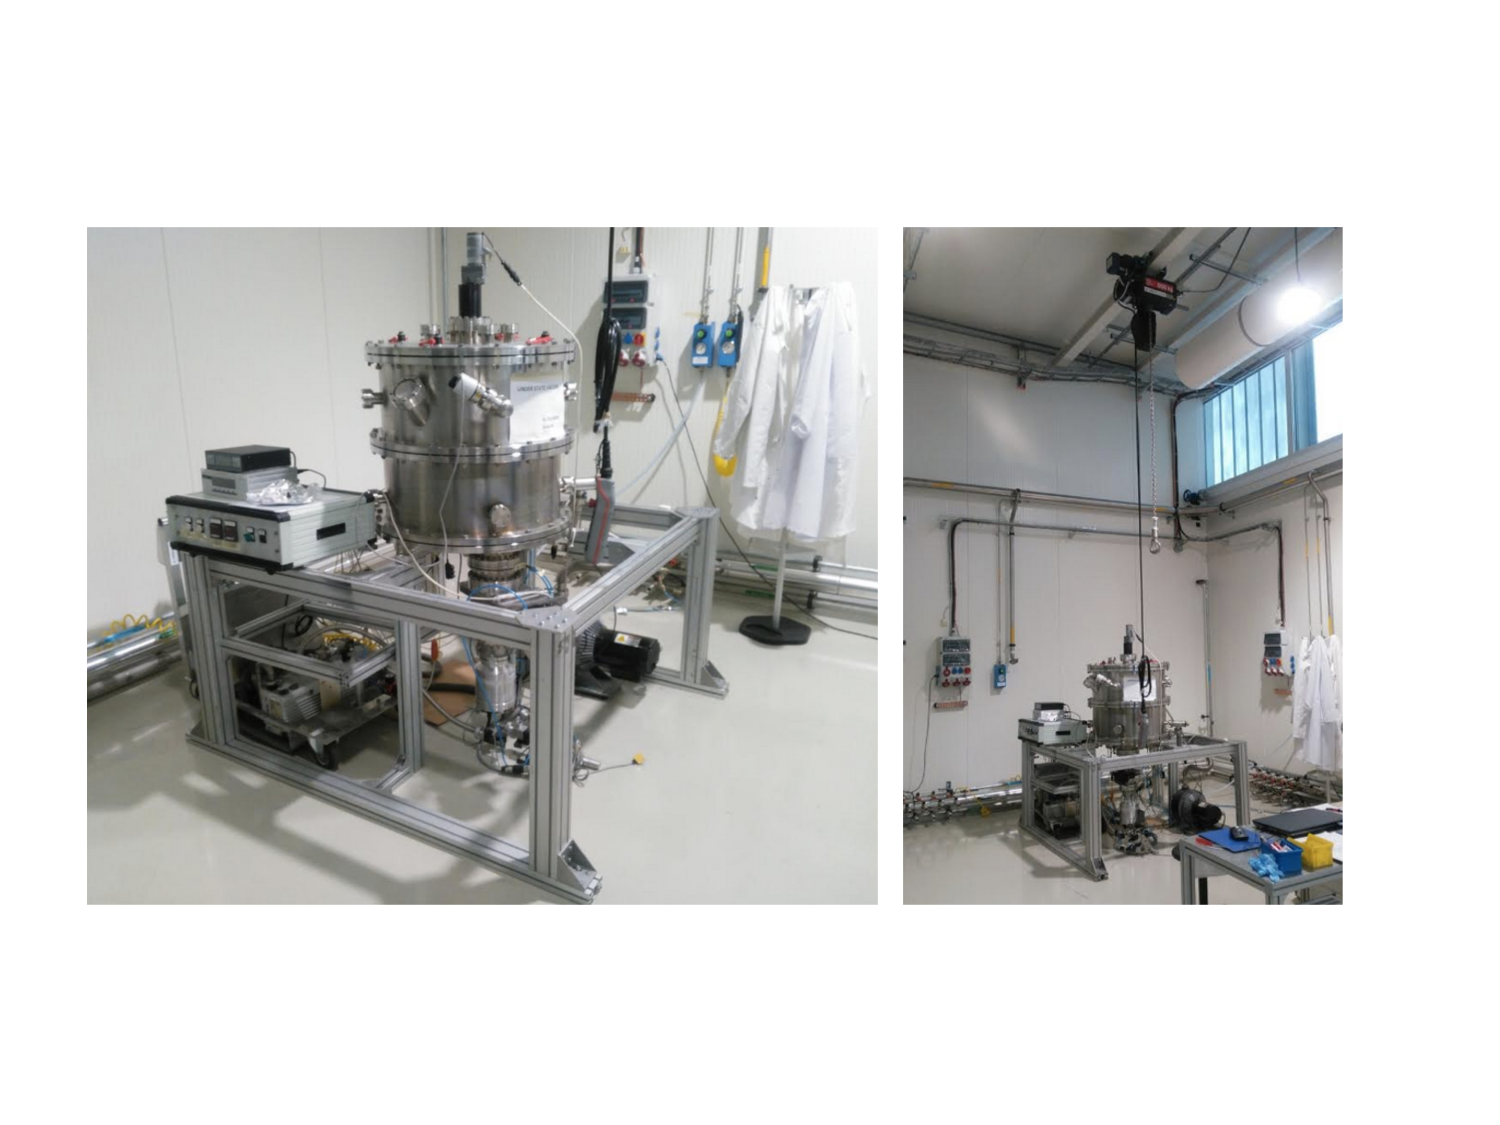
\includegraphics[width=0.8\textwidth]{dppd_11_4}
\end{dunefigure}

The \dwords{pmt} will be taken out of their individual cartons when they arrive at the \dword{ctsf}. The \dwords{pmt} will first be tested for basic functionality in their cartons to verify that they have been safely transported from the remote sites and will be kept in these boxes until the windows are coated. The \dword{pmt} windows will be cleaned with acetone and isopropanol before the evaporation. This will be done in the flow device/fume hood shown as a green box along the \SI{10}{\m} wall in Fig.~\ref{fig:dppd_11_3}. The gantry crane (indicated with red bars in Fig.~\ref{fig:dppd_11_3}) can move parts between the coating stations and the work desks. It will be used to remove the vessel lid and support it while the \dword{pmt} is installed for coating.

Following the evaporation procedure, an acrylic protective plates will be installed to cover the coated \dword{pmt} windows.
%, and the \dwords{pmt} will be placed in individual dark plastic protective bags. 
The \dwords{pmt} will be tested again for basic functionality. They will then be attached to the \num{4} $\times$ \num{3} structure for transportation to \surf.

At the \dword{ctsf}, the \dword{pmt} windows will be coated at a rate of \num{4} \dwords{pmt}/day or \num{20} \dwords{pmt}/week and \num{80} \dwords{pmt}/month. Given the installation rate of \num{120} \dwords{pmt}/month, the \dword{ctsf} operations should start before installation begins. \dword{ctsf} has sufficient storage capacity for the entire \dword{pmt} inventory of the \dword{pds}. 

\subsection{Underground Installation and Integration}
\label{subsec:dp-pds-undergroundinstallation}

The cryostat cable/fiber installation will precede the installation of the \dword{fc}. The cables/fibers will be routed from the flanges to the bottom of the cryostat. The total cable/fiber mass (length) is approximately \SI{50}{\kg} (\SI{25}{\m}) per sector with an average mass/length of \SI{2}{\kg/\m}, where one sector comprises \num{36} \dwords{pmt} (see Section~\ref{sec:dp-pds-overview_layout}). The free ends of the cables/fibers will be temporarily attached to the cryostat floor so they can be easily accessed during installation. The cable/fiber and tray installation will be done on both sides of the cryostat. At this stage, the \dword{hv} cables will be transported in a single box from the \dword{ctsf} to \surf. At the same time, a separate box containing \num{120} calibration fiber + fiber bundle assemblies will be transported from the \dword{ctsf} to \surf. The boxes will be transported to the cryostat roof so the cables/fibers can be hung through the feedthroughs for installation in the cable trays.  

Once the plastic wrap is removed, the \dword{pds} \dword{pmt} box and its entire contents can be moved to the clean room. The \dwords{pmt} will undergo functionality tests inside the custom design dark box, which can cover the entire structure of \num{4} $\times$ \num{3} \dwords{pmt}. The dark box will have a high voltage patch panel and allow consecutive tests of all \num{12} \dwords{pmt} in one testing session without intervention. The test will be a simple check for healthy \dword{pmt} operations. Once the operation of the \dwords{pmt} is verified, the structure can be moved into the cryostat.

Inside the cryostat, the \dwords{pmt} will be removed from the structure. %The window protections will be kept on the \dwords{pmt}. 
The \dwords{pmt} will be mounted on the membrane floor in the areas between the membrane corrugations using their support structures. The attachment is done using a stainless steel support base that can be point-glued to the membrane. The weight of the support and the \dword{pmt} exceeds the buoyancy force of the system. Furthermore, these supports also ensure stability against possible lateral forces acting on the \dwords{pmt} due to the liquid flow. Once the attachment is complete, the short \dword{hv} cables will be connected to the cold \dword{hv} cables with SHV barrel connectors. The calibration fibers will be routed and connected to the support structure. Once all the \dwords{pmt} of a given \dword{pds} sector are installed, the cables and fibers will be fixed in their final positions.

The installation will be done at a rate of \num{30} \dwords{pmt}/week. After installation, the empty \dword{pmt} boxes and the transport structures will be taken back to \dword{ctsf}.

Table~\ref{tab:dppd_t_11_1} summarizes the quantities related to the \dual \dword{pds} installation.

\begin{dunetable}
[Quantities related to the \dual \dword{pds} installation.]
{lc p{0.8\textwidth}}
{tab:dppd_t_11_1}
{Quantities related to the \dual \dword{pds} installation.}
Parameter & Value \\
Number of \dual \dword{pds} sectors	& \num{20} \\
Number of \dwords{pmt} per sector	& \num{36} \\
Number of calibration fibers per sector	& \num{6} \\
Number of feedthrough flanges per sector	& \num{1} \\
Total number of feedthrough flanges	& \num{20} \\
Number of \dword{hv} racks per sector	& \num{1} \\
Frequency of transportations to \surf from \dword{ctsf}	& \num{4} \dword{pds} boxes per month \\
Rate of installation	& \num{30} \dwords{pmt}/week \\
\end{dunetable}

The reflector/\dword{wls} panels will be assembled into a unit panel assembly on a dedicated table underground immediately prior to the installation following the procedure described in Section \ref{sec:dp-pds-mechanics}. They will be placed in a storage structure that can hold three regular and two extended reflector/\dword{wls} panel assemblies to be installed in one row of an \dword{fc} super-module. The installation of the panel assemblies will be synchronized with the installation of the \dword{fc} modules, which is described in Section \ref{sec:fddp-hv-transport-install} and depicted in Fig. ~\ref{fig:dp-super-module-installation-secuence}. Once a row of the \dword{fc} super-module is installed, the five reflector/\dword{wls} panel assemblies will be mounted on the FRP I-beams of the \dword{fc} submodules, starting from one end of the row and progressing towards the other. Figure \ref{fig:dppd_reflective_panel_installation_sequence} depicts the installation sequence of a unit reflector/\dword{wls} panel. The sequence can be described as below:

\begin{enumerate}
\item Put the top two screws accessing the back side through the top liquid flow opening (Fig.~ \ref{fig:dppd_reflective_panel_installation_sequence}  left).
\item Place two nuts in the closed holes of the long holding bar. Slide the long bar behind the panel to the level of the middle bar by holding it through the central liquid flow opening. Put the two middle bar screws and remove the long bar through the bottom liquid flow opening after sliding it all the way down (Fig.~ \ref{fig:dppd_reflective_panel_installation_sequence}  center).
\item Put the bottom two screws accessing the back side through the bottom liquid flow opening (Fig.~ \ref{fig:dppd_reflective_panel_installation_sequence}  right).
\end{enumerate}

\begin{dunefigure}[The schematic view of the installation sequence of a unit reflector/\dword{wls} panel assembly on the \dword{fc} I-beams.]{fig:dppd_reflective_panel_installation_sequence}
{The schematic view of the installation sequence of a unit reflector/\dword{wls} panel assembly on the \dword{fc} I-beams.}
\includegraphics[width=0.8\textwidth]{dppd_reflective_panel_installation_sequence}
\end{dunefigure}

\subsection{Commissioning}
\label{subsec:dp-pds-commissioning}

The commissioning of the \dword{pds} is performed in partitions. The size of a single partition will be mainly determined by the \dword{daq} and the \dword{hv} systems. The \dword{daq} and \dword{hv} partitions are commissioned, including the relevant control systems, before the \dwords{pmt} are connected to these systems.

The exact availability of the cryostat as a sufficiently dark environment depends on the overall installation schedule. Once it is possible, the \dwords{pmt} are powered up, and basic functionality and performance checks are carried out. These include pedestal data taking, i.e., recording event data with external periodic triggering, and tests with the calibration system where the data taking is triggered in synchronization with a light source, as described in Section \ref{sec:dp-pds-calibration}.

Basic performance characteristics of the \dwords{pmt}, e.g., the dark count rate and gain, will be validated with the commissioning tests. Issues related to installation can then be identified and eliminated. A commissioned sector becomes a part of the overall detector and can join the global calibration data taking and commissioning.



\section{Risks}
\label{sec:dp-pds-risks}

Table~\ref{tab:dppd_t_12_1} summarizes the risks associated with the \dual \dword{pds}. Severity level assigned for each risk is indicated as L (low), M (medium), and H (high). Below, we discuss these risks and mitigation plans for each risk item.

\begin{dunetable}
[Dual Phase Photon Detector Risk Summary]
{p{0.05\textwidth}p{0.7\textwidth}p{0.1\textwidth}}
{tab:dppd_t_12_1}
{Dual Phase Photon Detector Risk Summary.}
ID & Risk & Severity \\
1 & The photon detection system is not stable over the lifetime of the experiment (\dword{tpb}, channel) & L \\
2 & Implosion of \dwords{pmt} & L \\
3 & Fibers damaged during installation & L \\
4 & Background level (noise, light sources) is too high to distinguish signal & M \\
5 & \dword{pmt} signals are saturated & M \\
6 & Availability of resources for work at the installation/integration site is less than planned & M \\
7 & \dwords{pmt} damaged during shipment to the experiment site & M \\
8 & Not enough photons arriving to \dwords{pmt} & L \\
9 & Problems with choosing the correct type of screws and feedthroughs for the cabling and installation on the cryostat & M \\
10 & Excess noise due to poor grounding or not following grounding rules & M \\
11 & Problem with the connection of the cable to the \dword{pmt} base & L \\
12 & \dword{tpb} coating not sufficiently stable, contaminates \dword{lar} & L \\
\end{dunetable}

\begin{enumerate}

\item During \dword{fd} operation, the photon detection system could show performance fluctuations. For example, the \dword{pmt} gains could change. Continuous monitoring with the \dword{pmt} calibration system will enable us to resolve these issues individually for each \dword{pmt}.

\item Filling the detector with \dword{lar} could be a critical issue because a \dword{pmt} could implode. If this happens, the detector must be emptied. Special care must be taken during the filling of the detector with \dword{lar}. Pressure tests will be performed to quantify this.

\item Fibers are fragile and could be broken during installation because of the high number of fibers in the detector. Personnel in charge of assembling the different parts of the detector must take special care during fiber installation.

\item If external noise or light sources affect the \dwords{pmt}, measuring the signals without oscillations over the baseline could be difficult. Grounding, shielding, and power distribution are critical to the success of the experiment. Mitigation will require using proper shielding techniques on all cables and validating the noise performance of all equipment during installation and commissioning.

\item If we must increase the \dword{pmt} \dword{hv} to get higher gains, \dword{pmt} front-end inputs could be saturated. Then, we would lose a number of events during acquisition. To mitigate this risk, we will avoid operating the \dwords{pmt} at very high voltages. A balance between gain and saturation will be chosen.

\item The \dword{fd} construction cost estimate assumes that qualified local labor can be identified for certain activities. The cost will increase if external labor is required. Labor costs might need to increase to attract qualified candidates. Labor resources from laboratories may need to be housed and used. We will ensure that sufficient funding is available to move people temporarily from institutions involved in the \dword{pds} consortium to the integration/installation site.

\item If \dwords{pmt} are not packaged properly, they could be damaged during shipment. In this case, the \dword{pmt} cannot be used in the detector. We will use special packaging to avoid possible damage to the \dwords{pmt} during shipment. In any case, we will have a \num{10}\% contingency spare \dwords{pmt}.

\item Because of the long drift distance and the position of the cathode and ground grid on top of the \dwords{pmt}, the number of photons reaching the \dwords{pmt} might not be sufficient at some geometrical acceptances. Additional light collection enhancement tools are being considered to mitigate this effect. The most feasible option is to install wavelength shifting film on the inner surface of the \dword{fc}.

\item Choosing the wrong feedthrough means we could have higher noise levels or oscillations in the signals. Using the wrong parts might cause mechanical problems. Special care must be taken during the design of the screws and \dword{hv} feedthroughs needed for cabling in the detector. \dword{pddp} experience will be used to mitigate this risk.

\item While commissioning  the detector before \dword{lar} filling, excessive noise could appear because some components may fail because grounding rules are not observed. We will ensure that grounding rules are enforced and review any proposed modification of the detector design.

\item \dword{pmt} cables are soldered to the \dword{pmt} base and tested before installation. If the soldering is poorly done, some channels could show a bad waveform or no signal at all. Several tests will be done in the base before the \dwords{pmt} are installed: impedance, \dword{hv} tests in gas Ar to avoid sparks, and full test of the \dword{pmt} to verify signals are correct.

\item Limited past experience shows that the \dword{tpb} coating might not be sufficiently stable, possibly contaminating the \dword{lar} over the long term. We will carefully examine results from \dword{pddp} and other laboratory tests% as quickly as possible
. We will elaborate improved coating techniques if needed.

\end{enumerate}
\section{Safety}
\label{sec:dp-pds-safety}

The \dword{dp} \dword{pd} consortium will observe and comply with the institutional and national safety regulations of all of its production and assembly sites. The relevant safety documents for these sites will be reviewed by the consortium, and the regulations will be implemented by those responsible for local operations.

The production/assembly site is where \dword{hv} cables, \dword{hv} splitter boxes, calibration fibers, and the \dword{pmt} mechanics are prepared for final installation or assembly. The \dwords{pmt} are received, and the bases and mounting structures are connected to the \dwords{pmt}. The outputs of the production/assembly procedure are the \dwords{pmt} in their final mechanical and electronic structure. The assembly procedure requires several steps followed by specific \dword{qc} tests. The main safety risks during production are excessive heat from electrical and mechanical processing, chemicals for cleaning components, electrocution, and to some extent, heavy lifting and tripping hazards. Each production site host institution will develop dedicated handling, cleaning, and equipment procedures. The main safety risks during assembly are mechanical hazards such as sharp edges, heavy tools, and small parts. Procedures for using safety equipment, e.g.,  safety goggles, gloves, and safety shoes, will be developed by representatives of the production/assembly site institution. Delicate material handling and transportation instructions will also be developed by the institution. These instructions will be incorporated into the assembled structure for any downstream operation site.

The testing locations at the \dword{ctsf} and underground cleanroom  are responsible for the \dword{qc} of the assembled \dword{pmt} structure. These stations are also responsible for testing the \dword{hv} cables, \dword{hv} splitters, and the calibration fibers. The previously developed handling instructions will be respected during the testing procedures. Possible safety concerns are electrocution and heavy lifting. The functional tests of the \dwords{pmt} involve powering up the \dwords{pmt} for a predefined period. The testing procedures and the relevant safety regulations will be developed for and incorporated into all the future \dword{pmt} tests.

The production and assembly sites and the \dword{ctsf} also serve as transportation sites. The \dwords{pmt} are packed for transportation to the \dword{ctsf} and \dword{surf}. The contents of the transportation boxes are the individual cartons for the \dwords{pmt} with their bases, mounting assemblies, and short cables, placed into larger plastic pallet boxes in \num{4} $\times$ \num{3} $\times$ \num{3} arrays. % for transportation from the production/assembly sites to the \dword{ctsf}. 
Three stacked custom-design structures that can hold an array of 4$\times$3
\dwords{pmt}  will serve to transport \dwords{pmt}  from the \dwords{ctsf}  to \dwords{surf} in the same transportation boxes. 
At this stage, the main safety concern is the heavy lifting combined with the delicate detector handling procedures. 
Personnel to move the \num{36}-\dword{pmt} plastic pallet boxes both indoors and outside for truck loading will have special training. The loading and unloading procedures developed for the \dword{pmt} transportation boxes must be followed at the production and assembly sites, \dword{ctsf}, and at the ground and underground stations of the experiment site. Similar procedures will be developed for transporting the \dword{hv} cables and splitters, and calibration fibers.

The \dword{tpb} coating of the \dword{pmt} windows is done at the \dword{ctsf}, as described in Section~\ref{subsec:dp-pds-itf}. %The \dwords{pmt} are placed on shelves before they are removed from the transportation boxes, the windows will be cleaned, and \dword{tpb} evaporation will be done before the \dwords{pmt} are stored on shelves after the coating. The \dwords{pmt} will then go through functional testing and placed in their transportation assembly to be taken to the underground hall. 
The main safety risks at the \dword{ctsf} are electrocution, exposure to excessive heat and chemicals, and heavy lifting. Workplace safety regulations will be developed for the \dword{ctsf}. These will include general electrical and mechanical safety rules, as well as special handling instructions for the \dword{tpb} and other chemicals. Intense and continued exposure to \dword{tpb} and chemicals can cause temporary incapacitation e.g., eye, skin or respiratory irritation. We will implement carefully all the necessary safety measures. % from \dword{ppe}, to working schedule. % will be taken and implemented. 
Transporting the \dword{pmt} boxes in the \dword{ctsf} must follow the general safety regulations, and the gantry crane operator and others in the area must have the necessary training. The \dword{ctsf} will have proper interlocks, administrative and personnel control procedures, and monitoring at all times of its operation.

The underground operation and installation safety rules will follow general facility rules. The common risks at the underground cleanrooms, cryostat roof, and inside the cryostat are working in confined spaces and oxygen deficiency hazard. The \dword{dp} \dword{pds}-specific risks include electrocution for pre-installation testing, heavy lifting, and tripping.

Safety is the highest priority at all stages of  \dword{dp} \dword{pds} operations. The safety procedures are developed by the particular institutions involved in specific operations and are discussed and approved by the consortium. The guidelines and procedures for handling and transportation of the  \dword{dp} \dword{pds} materials will be made part of the \dword{ctsf} and underground facility safety regulations.
\section{Project Management}
\label{sec:dp-pds-management}

The \dual \dword{pd} consortium was formed in 2017 and it is composed of eleven institutes from France, Peru, Spain, UK and USA. The charge of the \dual \dword{pd} consortium is to plan and execute the construction, installation and commissioning of the \dword{dp} \dword{pds}.
% I think we should check with Peru and UK if they are still interested in being included in the consortium

%%%%%%%%%%%%%%%%%%%%%%%%%%%%%%%%%
\subsection{Consortium Organization}

The current \dual \dword{pd} consortium Leader (CL) is %In\'{e}s Gil-Botella
 from CIEMAT (Spain) and the Technical Lead (TL) is %Dominique Duchesneau 
 from LAPP (France). They are members of the \dword{dune} Technical Board and they represent the consortium to the overall \dword{dune} collaboration. The CL is responsible for the subsystem deliverables and for the effective management of the consortium. The TL acts as the overall project manager and is the interface to the International Project Office (IPO); he is responsible for monitoring and reporting on progress with respect to the agreed schedule and for issues related to interface documentation.

The institutions participating in the consortium are responsible for the design or construction of a particular subsystem. It is hoped that the national groups within the consortia will be able to approach relevant funding agencies with a specific construction-phase proposal, such that a likely funding line can be established in or before 2019. The \dual \dword{pd} consortium is open to any new institution willing to join the current effort.

The current institutions participating in the \dual \dword{pd} consortium are LAPP (France); PUCP (Peru); IFAE, CIEMAT, and IFIC (Spain); UCL (UK); and ANL, Duke U., U. of Iowa, SDSMT, and UTA (USA).

The \dual \dword{pd} consortium is divided into four working groups: photosensors and electronics, calibration system, mechanics and integration, and simulation and physics. The corresponding current WG convener institutions are:
\begin{itemize}
% AH REMOVING NAMES
\item WG1: Photosensors and Electronics -  CIEMAT %A. Verdugo
\item WG2: Calibration System -  CIEMAT %C. Cuesta
\item WG3: Mechanics and Integration - U. of Iowa %B. Bilki 
\item WG4: Sim. \& Phys. - %K. Scholberg (
Duke U., %M. Sorel (
IFIC, %L. Zambelli (
LAPP
\end{itemize}

%%%%%%%%%%%%%%%%%%%%%%%%%%%%%%%%%
%\subsection{Planning Assumptions}
%\label{sec:fddp-pd-12.2}

%The optimization and final design of the \dual \dword{pd} system will be driven by the \dword{pddp} data, expected by Summer 2019.

%\dword{pddp} operation and data analysis are fundamental steps to understanding whether the current \dword{pds} design considered as baseline, based on cryogenic \dwords{pmt} with \dword{tpb} coating, is able to provide $t_0$ for non-beam events, background rejection and triggering on non-beam events. These data will be used to tune the \dword{mc} simulations and extrapolate the performance of the system to the \dword{dpmod}.

%%%%%%%%%%%%%%%%%%%%%%%%%%%%%%%%%
\subsection{WBS and Institutional Responsibilities}

The \dual \dword{pd} consortium has developed a detailed breakdown of deliverables and responsibilities included in the overall \dword{dune} collaboration \dword{wbs}~\cite{bib:docdb5594} coordinated by the IPO. The main deliverables are %based on the \dword{pddp} \dword{pds}  and are 
divided into seven topics. These are listed along with the participating institutions below: 

%\dword{pddp} \dword{pds} 
\begin{enumerate}
\item Management \dual \dword{pds} (includes milestones and review dates) \textit{- LAPP, CIEMAT }
\item Physics and Simulations \textit{- Duke, LAPP, IFIC, SDSMT, CIEMAT, PUCP, UCL, Texas-Austin}
\item Design, Engineering, R\&D and validation tests \textit{- Iowa, CIEMAT, IFIC, UCL, Texas-Austin, IFAE, SDSMT}
\item Production Setup (includes tooling) \textit{- UCL}
\item Production (includes component production, assembly, testing, and \dword{qc}) \textit{- Iowa, CIEMAT, IFAE, IFIC, UCL, Texas-Austin, Duke, SDSMT, LAPP}
\item Integration (contributions to activities at global integration facility) \textit{- SDSMT}
\item Installation (contributions to activities at \surf) \textit{- CIEMAT, IFIC, SDSMT, Iowa}
\end{enumerate}

\subsection{High Level Schedule}

%The \dual \dword{pds} consortium's main activities during the next \num{16} months are focused on developing the \dword{tdr}. 
The main high-level milestones are detailed in Table~\ref{tab:dppd_t_12_5} for the pre-\dword{tdr} period. The plan for the activities in the post-\dword{tdr} period is summarized in Table~\ref{tab:dppd_t_12_6}.

\begin{dunetable}
[Pre-\dword{tdr} key milestones]
{|l|l| p{0.8\textwidth}}
{tab:dppd_t_12_5}
{Pre-\dword{tdr} key milestones (TO BE UPDATED)}

Milestone & End date \\ \toprowrule
Simulations and physics: %Finalize the 
Implementation of \dual optical & \\
simulation in \larsoft for \dword{pddp} & 08/2018 \\ \colhline
Simulations and physics: Optimization of the & \\
\dword{dpmod} performance to fulfill the physics requirements and & \\
definition of a trigger strategy & 05/2019 \\ \colhline
Photosensors: Components selection and final design & 03/2019 \\ \colhline
\dword{pmt} calibration system design and selection of components & 03/2019 \\ \colhline
Cabling definition and design of flange & 03/2019 \\ \colhline
Design review in light of \dword{pddp} calibration data & 03/2019 \\ \colhline
\dword{qc} plan & 06/2018 \\ \colhline
Identification of Interfaces & 06/2018 \\ \colhline
Integration, installation and commissioning plans & 12/2018 \\ \colhline
\dword{dpmod} \dword{tdr} & 06/2019 \\ 
\end{dunetable}

\fixme{Remove table with pre-TDR milestones, Tab.~\ref{tab:dppd_t_12_5}?}

\begin{dunetable}
[Post-\dword{tdr} key milestones]
{|l|l|l| p{0.8\textwidth}}
{tab:dppd_t_12_6}
{Post-\dword{tdr} key milestones}

Milestone & Start date & End date \\ \toprowrule
\textbf{\dword{pmt} preparation and installation} (can be done in batches) & & \\ \colhline
\dword{pmt} procurement procedure and production & 01/2021 & 12/2022 \\ \colhline
\dword{pmt} base design and manufacturing & 01/2022 & 12/2022 \\ \colhline
\dword{pmt} support structure production and assembly & 08/2022 & 01/2023 \\ \colhline
\dword{pmt} characterization - \num{10} \dwords{pmt}/week (two facilities) & 02/2023 & 12/2023 \\ \colhline
\dword{tpb} coating (two facilities similar to that for CERN ICARUS) & 01/2024 & 12/2024 \\ \colhline
Splitter production and tests & 05/2024 & 12/2024 \\ \colhline
\textbf{Installation at \surf} & & \\ \colhline
\dword{pmt} cable and fiber routing in cryostat from flange to bottom & & \\
                  (depends on \dword{fc} and flange installation) & 09/2024 & 09/2024 \\ \colhline
\dword{pmt} testing, installation in cryostat and cabling (\num{72} \dwords{pmt}/month) & 10/2024 & 07/2025 \\ \colhline
\dword{pmt} support installation on the membrane & & \\
                  (in parallel by sector with \dword{pmt} installation) & 10/2024 & 07/2025 \\ \colhline
Splitter installation & & \\
                  (in parallel with \dword{pmt} installation to test cabling and connections) & 10/2024 & 07/2025 \\ \colhline
\textbf{Light calibration system} & & \\ \colhline
Fibers, light source tests and procurement & 06/2023 & 05/2024 \\ \colhline
Fiber calibration system installation & & \\
                  (in parallel with \dword{pmt} installation with validation test) & 09/2024 & 07/2025 \\ 
\end{dunetable}

\fixme{Update Tab.~\ref{tab:dppd_t_12_6} according to new schedule, with installation of 2nd module starting on 08/2025.}

\subsection{High Level Cost of Baseline Design}

An initial cost estimate of the \dual \dword{pd} photon detection system for one 10kt DUNE detector was developed in 2018 (Table~\ref{tab:dppd_t1.7}). This is based on protoDUNE-DP costs.

\begin{dunetable}
[Dual Phase Photon Detection System Cost Summary]
{|l|l| p{0.8\textwidth}}
{tab:dppd_t1.7}
{Dual Phase Photon Detection System Cost Summary (TO BE COMPLETED)}

Item & Core Cost (k\$ US)\\ \toprowrule
Item 1 & 1.0 \\
Item 2 & 1.0 \\
Item 3 & 1.0 \\
... & ... \\
\end{dunetable}

\fixme{Complete costs table, Tab.~\ref{tab:dppd_t1.7}.}
\newpage

\section{Appendix - Alternatives}
\label{sec:dp-pds-appendix}

\subsection{Individual Ground Grids}
\label{sec:dp-pds-appendix-grid}

In collaboration with the \dword{hv} consortium, the installation of individual ground grids for each \dword{pmt} in place of the ground grid table structure is under consideration. Since the individual ground grid cages will potentially have thinner wires and will be closer to the \dword{pmt} windows, generating a smaller shadow, they should increase the acceptance of the \dwords{pmt}.

The feasibility of the design in operation under \dune \dual conditions will be studied by the \dword{hv} consortium. The design of the individual grids will be developed as a common effort of the two consortia engineering teams. The \dword{hv} consortium will produce the grids. The grids will be installed at the \dword{ctsf} by \dual \dword{pd} consortium. The \dwords{pmt} will be installed with their individual grid cages by \dual \dword{pd} consortium. 

\subsection{Calibration System Alternatives}
\label{sec:dp-pds-appendix-calibration}

Alternatives to the baseline design of the calibration system described in Section~\ref{sec:dp-pds-calibration} will be pursued with R\&D measurements to make the system more effective, reduce the cost, and mitigate issues related to scaling to the \dune \dual size. These alternatives include reducing the number of fibers, studying other options for the reference sensor, and increasing the input light if necessary. To reduce the number of fibers, light diffusers can be used, so that one fiber can illuminate at least four \dwords{pmt}. For instance, a diffuser could be placed at the ground grid, or in the case of individual ground grids, on the side walls. With the same aim of reducing the total number of fibers, an alternative calibration system with two fibers placed at the top of the field cage is being tested in \dword{pddp}, so that one fiber can illuminate several \dwords{pmt}. Other than the diffusers and fiber placement, considered alternatives are related to the external system and can be implemented with minimal interference with other subsystems.

\subsection{Xe Doping of Liquid Argon}
\label{sec:dp-pds-appendix-xedoping}

Doping the \dword{lar} volume with Xe is an attractive option in terms of providing a volume distributed wavelength shifting. Major advantages of Xe doping are triggering the long-lived triplet argon excimer to produce a faster signal reducing the fraction of late light; shifting the scintillation signal to longer wavelengths (\SI{175}{nm}) and as a consequence, a longer Rayleigh scattering length.

Dedicated simulations on light yield in the full \dword{dp} \dword{fd} cryostat in the presence of Xe doping were performed. Figure~\ref{fig:dppd_fd_light_yield_xedoping} shows the 1D light yields as a function of the drift (transverse) direction in the left (right) panel, averaging over the other two spatial coordinates. It is evident that the Xe doping can be considered as an immediate alternative to the baseline design with half coverage reflector/\dword{wls} panels in terms of light output. On the other hand, keeping a smaller area coverage reflector/\dword{wls} panels closer to the charge readout may be preferable in order to improve the uniformity.

%\subsection{Wavelength Shifting Reflective Foils}
%\label{sec:dp-pds-appendix-wlsfoils}

%To enhance light collection and improve response uniformity in the detector volume, installing wavelength shifting reflector foils on the \dword{fc} inner surfaces is under consideration. This alternative is being evaluated for two particular cases: covering \dword{fc} inner walls fully with the foils and covering only the upper half of the \dword{fc} with the foils. In addition to completely evaluating the effect on physics within the consortium, the interface, particularly the effect on liquid circulation, the effective electric field, and the mechanical structure are being discussed with the \dword{hv} consortium.

%\fixme{If included in the baseline design, move to section \ref{sec:dp-pds-mechanics}}

\begin{dunefigure}[Expected 1D light yields in the full \dshort{dpmod} with xenon doping]{fig:dppd_fd_light_yield_xedoping}
{Expected light yield in the full \dword{dp} \dword{fd} cryostat in the presence of xenon doping. The yield units are number of photo-electrons per \si{\MeV} of deposited energy. The 1D yields are shown as a function of the drift (transverse) direction in the left (right) panel, averaging over the other two spatial coordinates (not shown), similarly to Figure~\ref{fig:dppd_fd_light_yield_comparisons}. The three histograms correspond to the half foil baseline design without xenon doping, and to two no foil geometries, with and without xenon doping, respectively.}
\raisebox{0.1cm}{\includegraphics[width=0.49\textwidth]{graphics/dppd_xedoping_drift.png}} \hfill
\includegraphics[width=0.49\textwidth]{graphics/dppd_xedoping_transverse.png}
\end{dunefigure}